%% equivalence.tex - Polynomial-time kernel reductions
%%
%% Copyright 2010, 2011, 2012, 2014 Jeffrey Finkelstein.
%%
%% This LaTeX markup document is made available under the terms of the Creative
%% Commons Attribution-ShareAlike 4.0 International License,
%% https://creativecommons.org/licenses/by-sa/4.0/.
\documentclass{article}

%% This must come before hyperref.
\usepackage{amsthm}
%% These must come before hyperref.
\usepackage{thmtools}
\usepackage{thm-restate}
%% This must come before complexity.
\usepackage{hyperref}
%% This is strongly recommended by biblatex.
\usepackage[english]{babel}
%% This must come before csquotes.
\usepackage[utf8]{inputenc}
%% This is strongly recommended by biblatex.
\usepackage{csquotes}
\usepackage[backend=biber]{biblatex}
\usepackage{amsmath}
\usepackage{amssymb}
\usepackage{complexity}
\usepackage{textcomp} % for \textlangle, \textrangle
%% This is required by draftwatermark.
\usepackage{type1cm}
\usepackage[firstpage]{draftwatermark}
\usepackage{tikz}
\usepackage{microtype}

%% Set the amount by which certain characters protrude into the margins.
\LoadMicrotypeFile{cmr}
\SetProtrusion
    [load=cmr-OT1]
    {encoding=OT1, family=cmr}
    {
      \textquotedblright = {,1000},
      {]} = {,1000},
      {,} = {,1000},
      . = {,1000}
    }

\SetWatermarkLightness{0.9}
\SetWatermarkText{Work-in-progress}
\SetWatermarkFontSize{3.5cm}

\hypersetup{pdftitle={Polynomial time kernel reductions}, pdfauthor={Jeffrey Finkelstein}}

\addbibresource{equivalence.bib}

\declaretheorem[numberwithin=section]{theorem}
\declaretheorem[numberlike=theorem]{claim}
\declaretheorem[numberlike=theorem]{lemma}
\declaretheorem[numberlike=theorem]{proposition}
\declaretheorem[numberlike=theorem]{corollary}
\declaretheorem[numberlike=theorem, style=definition]{construction}
\declaretheorem[numberlike=theorem, style=definition]{definition}
\declaretheorem[numberlike=theorem, style=definition, name=Open problem]{openproblem}
\declaretheorem[numberlike=theorem, style=definition]{example}
\declaretheorem[numberlike=theorem, style=definition]{remark}

% create a proof sketch environment
\newenvironment{sketch}{\begin{proof}[Proof sketch]}{\end{proof}}

% custom shortcut commands
%\newcommand{\email}[1]{\href{mailto:#1}{\nolinkurl{#1}}} % formatting emails
\newcommand{\email}[1]{\textlangle\href{mailto:#1}{\nolinkurl{#1}}\textrangle}
\newcommand{\plain}[1]{\text{ #1 }} % plain text inside math environments
\newcommand{\sigmastar}{\{0, 1\}^{*}} % the set of all binary strings
\newcommand{\kj}{\overset{ker}{\oplus}} % kernel join
\newcommand{\nkr}{\nleq^{P}_{ker}} % kernel-reduces
\newcommand{\kr}{\leq^{P}_{ker}} % kernel-reduces
\newcommand{\pot}{\leq^{P}_{pot}} % potentially reduces
\newcommand{\npot}{\nleq^{P}_{pot}} % does not potentially reduce
\newcommand{\krnt}{\leq_{ker}} % kernel-reduces without time bound
\newcommand{\nkrnt}{\nleq_{ker}} % does not kernel-reduce without time bound
\newcommand{\kri}{\leq^{P}_{ker,1\text{--}1}} % 1-1 kernel-reduces
\newcommand{\mor}{\leq^{P}_{m}} % many-one reduces
\newcommand{\mornt}{\leq_m}
\newcommand{\moe}{\equiv^{P}_{m}} % many-one equivalent
\newcommand{\lb}{\left\{} % left curly brace for set notation
\newcommand{\rb}{\right\}} % right curly brace for set notation
\newcommand{\st}{\,\middle|\,} % ``such that'' pipe, for use in set definitions
\newcommand{\symdiff}{\bigtriangleup} % set symmetric difference
\newcommand{\defn}[1]{\emph{#1}} % emphasize words which are being defined
\newcommand{\pair}[2]{\left\langle#1,#2\right\rangle} % pairing function
\newcommand{\triple}[3]{\left\langle#1,#2,#3\right\rangle} % tripling function
%% \newcommand{\Q}{\textsf{Q}} % to represent an unknown quantifier
%% \newcommand{\QBF}{\lang{QBF}} % the language QBF
%% \newcommand{\QBFEq}{\lang{QBFEq}} % the language of equivalent QBFs
\newcommand{\todo}[1]{\textbf{TODO #1}}

% redefine footnote so it has no reference and no number
\long\def\symbolfootnote#1{\begingroup%
\def\thefootnote{\fnsymbol{footnote}}\footnotetext{#1}\endgroup} 

% define the author, title, and date
\author{Jeffrey~Finkelstein\\ Computer Science Department, Boston University
  \and Benjamin~Hescott\\ Computer Science Department, Tufts University}
\title{Polynomial time kernel reductions}

\begin{document}

\maketitle

In this paper we analyze the notion of kernel reductions among equivalence
problems, as defined in Fortnow and Grochow. We first examine what kernel
reductions look like, practically, among feasible equivalence problems. We next
provide some evidence that the restriction of a polynomial time kernel
reduction is not on the time complexity of the reduction, but on the number of
equivalence classes in the equivalence relations being reduced. We then examine
the graph isomorphism problem and problems equivalent to it under polynomial
time many-one reductions, and find that of these problems the ones which are
equivalence problems are in fact equivalent to the graph isomorphism problem
under polynomial time kernel reductions.

%% copyright.tex - the copyright notice for this paper
%%
%% Copyright 2010, 2011, 2012, 2014, 2015 Jeffrey Finkelstein.
%%
%% This LaTeX markup document is made available under the terms of the Creative
%% Commons Attribution-ShareAlike 4.0 International License,
%% https://creativecommons.org/licenses/by-sa/4.0/.
\symbolfootnote{%
  Copyright 2010, 2011, 2012, 2014, 2015 Jeffrey~Finkelstein and Benjamin~Hescott.

  This document is licensed under the Creative Commons Attribution-ShareAlike 4.0 International License, which is available at \mbox{\url{https://creativecommons.org/licenses/by-sa/4.0/}}.
  The \LaTeX{} markup that generated this document can be downloaded from its website at \mbox{\url{https://github.com/jfinkels/equivalence}}.
  The markup is distributed under the same license.
}


%% introduction.tex - introduction and motivation for the work
%%
%% Copyright 2010, 2011, 2012, 2014, 2015 Jeffrey Finkelstein.
%%
%% This LaTeX markup document is made available under the terms of the Creative
%% Commons Attribution-ShareAlike 4.0 International License,
%% https://creativecommons.org/licenses/by-sa/4.0/.
\section{Introduction}
% Foreword
%
% context (focus on anyone) why now? - current situation, and why the need is so important
Our main tool for comparing relative difficulties of computational problems is the many-one reduction, an encoding of an instance of one problem as an instance of another.
% need (focus on readers) why you? - why this is relevant to the reader, and why something needed to be done
Reductions involving problems of equivalence like the graph isomorphism problem have access to both elements of the pair simultaneously.
However, a more natural notion of reduction between problems of equivalence requires the reduction to access each element of the pair separately, and indeed, to the best of our knowledge, every many-one reduction between problems of equivalence behaves this way.

%%% relevant existing work, given as part of the need
The \emph{kernel reduction}, defined in \autocite[Definition~4.13]{fg11}, formally captures this notion of reduction among computational problems of equivalence involving independent transformation of each element of a pair.
This type of reduction has appeared not only in complexity theory but also in computability theory and mathematical logic under names such as ``Borel reduction'' \autocite{fs89}, ``strong isomorphism reduction'' \autocite{bcffm}, and ``functorial reduction'' \autocite{babai14, babai77, kucera76, zkt85}, among many others.
What are the limitations of these types of reductions?

% task (focus on author) why me? - what was undertaken to address the need
We undertake a thorough investigation of the basic properties of kernel reductions, comparing them with the basic properties of many-one reductions.
% object (focus on document) why this document - what the document covers
%% The starting point for understanding many-one reductions is $\P$ and $\NP$, so we attempt to extend the definition from \autocite{fg11} of $\PEq$, the class of equivalence problems decidable in polynomial time, to the definition of the complexity class $\NPEq$ (\autoref{sec:definitions}).
We discover sufficient conditions for complete problems under kernel reductions in classes of equivalence problems (\autoref{sec:generalcompleteness}).
We compare the new notion of completeness under kernel reductions with the usual notion of completeness under many-one reductions (\autoref{sec:npeqcompleteness}).
We prove, under the assumption that $\P \neq \NP$, the existence of $\NPEq$-intermediary problems with respect to kernel reductions (\autoref{sec:intermediary}).
Finally, we determine the limitations of kernel reductions; these appear to be combinatorial, not computational, in nature (\autoref{sec:limitations}).

% Summary
%
% findings (focus on author) what? - what the work revealed when performing the task
We find that kernel reductions are essentially similar to many-one reductions, but differ in some key aspects.
Like many-one reductions, kernel reductions are transitive and have good closure properties.
The class of equivalence problems in $\PSPACE$ has a complete problem under kernel reductions (\autoref{cor:hardproblems}).
The equivalence of the two equalities $\P = \NP$ and $\PEq = \NPEq$ (\autoref{thm:pnppeqnpeq}) can be proven using the similarity between many-one and kernel reductions.
Just as many-one reductions allow the existence of $\NP$-intermediary problems, kernel reductions allow for the possibility of $\NPEq$-intermediary problems (\autoref{thm:intermediary}).
On the other hand, there are equivalence relations between which there is a many-one reduction but no kernel reduction (\autoref{thm:different}).
Specifically, if there are more equivalence classes, up to strings of certain lengths, in one equivalence relation than in the other, then no kernel reduction can exist.
Finally, under some assumptions, there is an equivalence problem that is not complete for $\NPEq$ under injective kernel reductions (\autoref{thm:inj}), whereas nearly every known $\NP$-complete problem is isomorphic (the Berman--Hartmanis conjecture \autocite{bh77} states that \emph{every} $\NP$-complete problem is isomorphic).

% conclusion (focus on readers) so what? - what the findings mean for the audience
The techniques used in this paper to show that kernel reductions are weaker than many-one reductions are combinatorial (for example, comparing the numbers of equivalence classes).
Combining these with other complexity theoretic and algebraic techniques has already proven useful: there is no polynomial-time kernel reduction from the graph isomorphism problem to the isomorphism problem for strongly regular graphs \autocite[Theorem~22]{babai14}.
This is interesting because even though the latter appears to be a difficult problem, no polynomial-time many-one reduction from the former to the latter is expected to exist \autocite{babai14}, and the lack of a kernel reduction is evidence in that direction.

% perspective (focus on anyone) what now? - what should be done next
Besides the open problems listed in \autoref{sec:generalcompleteness}, here are several interesting questions we have not examined.
What do problems of \emph{inequivalence} (see \autocite{gj79} for some examples) have to do with completeness under kernel reductions?
When can we translate a proof that an equivalence relation is complete under many-one reductions (see \autocite[Theorem~1]{rs11} for a recent example) to a proof that it is complete under kernel reductions?
When is the problem of computing the size of an equivalence class Turing-equivalent to deciding equivalence (see \autocite[Theorem~1.24]{kst93} for an example of such an equivalence for graph isomorphism).

%% preliminaries.tex - mathematical definitions of kernel reductions
%%
%% Copyright 2010, 2011, 2012, 2014 Jeffrey Finkelstein.
%%
%% This LaTeX markup document is made available under the terms of the Creative
%% Commons Attribution-ShareAlike 4.0 International License,
%% https://creativecommons.org/licenses/by-sa/4.0/.
\section{Preliminaries}
\label{sec:preliminaries}

If $f\colon S\to T$ is a well-defined function and $S'\subseteq S$, then \defn{$f$ restricted to the domain $S'$} is the function $f'\colon S'\to T$ defined by $f'(x)=f(x)$ for all $x\in S'$.
We denote this restricted function on a smaller domain by $f|_{S'}$.
The \emph{image of $S'$}, denoted $f(S')$, is defined by $f(S') = \{f(s) \, | \, s \in S'\}$.

In this paper, $\Sigma$ denotes the binary alphabet $\{0, 1\}$.
$\Sigma^*$ is the set of all binary strings over the alphabet $\Sigma$ and $\Sigma^{\leq n}$ is the set $\lb w\in\Sigma^* \st |w|\leq n \rb$.
The empty string will be denoted by $\lambda$.
If $\sigma\in\Sigma$ then $\sigma^k$ is the string consisting of $k$ concatenated copies of the symbol $\sigma$.
If $x$ and $y$ are elements of $\Sigma^*$, then we denote by $\pair{x}{y}$ the \defn{pairwise encoding} of $x$ and $y$, which is itself an element of $\Sigma^*$.
In this paper, we will assume the reasonable pairwise encoding defined by $\pair{x}{y}=x_1x_1x_2x_2\cdots x_{|x|}x_{|x|}01y_1y_1y_2y_2\cdots y_{|y|}y_{|y|}$ for all $x$ and $y$ in $\Sigma^*$.
As usual, a \defn{language} over an alphabet $\Sigma$ is a subset of $\Sigma^*$.
The \defn{complement} of a language $L$ is $\Sigma^*\backslash L$, and is denoted $\overline{L}$.

The complexity classes $\P$, $\NP$, $\FP$ (polynomial time computable functions), $\SKP$, $\PKP$, $\DKP$, and $\PSPACE$ have the usual definitions.
The set of words accepted by a Turing machine $M$ is denoted $L(M)$.
The \defn{complement} of a complexity class $\mathcal{C}$ is the set of complements of languages in $\mathcal{C}$, and is denoted $\coC$.

We say a Turing machine $M$ is a \defn{polynomially clocked Turing machine} if the description of $M$ includes a positive integer $k$ such that $M$ halts within time $kn^k$ on all inputs of length $n$.

If $L_1$ and $L_2$ are languages, we say that \defn{$L_1$ many-one reduces to $L_2$} if there exists a computable function $f$ such that $w \in L_1$ if and only if $f(w) \in L_2$.
We denote this by $L_1 \mornt L_2$.
If $f$ is computable in polynomial time, we denote this by $L_1 \mor L_2$.
%% If $L_1 \mor L_2$ and $L_2 \mor L_1$, we say that $L_1$ and $L_2$ are \defn{equivalent under polynomial time many-one reductions}, and denote this by $L_1\moe L_2$.

A set $R \subseteq \Sigma^* \times \Sigma^*$ is an \defn{equivalence relation on $\Sigma^*$} if $R$ satisfies the following three properties.
\begin{itemize}
\item (reflexivity) For all $x \in \Sigma^*$, $(x,x)\in R$.
\item (symmetry) For all $x,y\in \Sigma^*$, $(x,y)\in R$ implies $(y,x)\in R$.
\item (transitivity) For all $x,y,z\in \Sigma^*$, $(x,y)\in R$ and $(y,z)\in R$ implies $(x,z)\in R$.
\end{itemize}
An equivalence relation $R$ can be encoded as a language by taking the pairwise encoding of each pair in $R$.
In this way we can study the computational complexity of classes of languages which represent equivalence relations.
In this paper we will abuse notation and write $\pair{x}{y}\in R$ for an equivalence relation $R$ on $\Sigma^*$, but what we really mean is $(x,y)\in R$ and $\pair{x}{y}\in L_R$, the language on the alphabet $\Sigma$ induced by $R$.

The \defn{equivalence class} of $x$ with respect to an equivalence relation $R$ on $\Sigma^*$ is $\lb y\in \Sigma^* \st (x,y)\in R \rb$.
It is denoted $[x]_R$, or if the context is clear, simply $[x]$.
Each element $x\in \Sigma^*$ is in exactly one equivalence class, so the equivalence classes of an equivalence relation on $\Sigma^*$ provide a partition of $\Sigma^*$.
Conversely, a partition of $\Sigma^*$ induces an equivalence relation on $\Sigma^*$ in which a pair of elements is in the relation if they are in the same block of the partition.

A \defn{complete invariant} for an equivalence relation $R$ on $\Sigma^*$ is a function $f\colon \Sigma^*\to T$ such that for all $x,y\in \Sigma^*$, $(x,y)\in R$ if and only if $f(x)=f(y)$.
%% (In other words, a complete invariant is a kernel reduction from $R$ to the equality relation.)
In \autoref{sec:definitions} we will define generalizations of the complete invariant which accept as input an additional witness to the equivalence of $x$ and $y$.

\defn{$\PEq$} is the class of equivalence relations for which membership can be decided by a Turing machine running in deterministic polynomial time.
\defn{$\NPEq$} is the class of equivalence relations for which membership can be decided by a Turing machine running in non-deterministic polynomial time.
In other words, $\PEq$ is the set of (languages induced by) equivalence relations which are in \P, and $\NPEq$ is the set of (languages induced by) equivalence relations which are in \NP.
In general, the class \defn{$\CEq$} is the class of languages induced by equivalence relations which are in the complexity class $\mathcal{C}$.
As usual, $\PEq\subseteq\NPEq$.
%\defn{$\Ker$} is the class of equivalence relations which have a polynomial time computable complete invariant.

We now require a natural notion of reduction among equivalence relations.
If $R$ and $S$ are equivalence relations on $\Sigma^*$, we say $R$ \defn{kernel reduces to} $S$ if there exists a computable $f\colon\Sigma^*\to\Sigma^*$ such that $\forall x,y\in\Sigma^*$, $\pair{x}{y}\in R\iff \pair{f(x)}{f(y)}\in S$.
We denote this by $R\krnt S$.
If $f$ is computable in polynomial time, then we say $R$ \defn{polynomial time kernel reduces to} $S$ and use the notation $R\kr S$.

Notice the difference between a kernel reduction and a plain old many-one reduction: a kernel reduction maps $\pair{x}{y}\in R$ to $\pair{f(x)}{f(y)}\in S$, whereas a many-one reduction maps $\pair{x}{y}\in R$ to $f(\pair{x}{y})\in S$, for some polynomial time computable function $f$.
Informally, a function which computes a many-one reduction has access to both $x$ and $y$ but a function which computes a kernel reduction has access to only one of $x$ and $y$ at a time.
Since it is more restrictive, a kernel reduction induces a many-one reduction (namely the function $\pair{x}{y} \mapsto \pair{f(x)}{f(y)}$).
Still, kernel reductions compose just as many-one reductions do, and $\NPEq$ is closed under polynomial time kernel reductions, allowing us to adapt existing complexity theoretic analysis to the study of complexity of equivalence relations.

As an analog to polynomial time many-one completeness in \NP, we define a similar notion of completeness under polynomial time kernel reductions in \NPEq.
An equivalence relation $S$ is \defn{\NPEq-hard} if for all $R\in\NPEq$, $R\kr S$.
If $S$ is also in \NPEq, then it is \defn{\NPEq-complete}.
If $S$ is \NPEq-complete, we sometimes say that $S$ is \defn{complete under $\kr$ reductions in \NPEq}.
Generally, an equivalence relation $S$ is \defn{$\CEq$-hard} if for all $R\in\CEq$, $R\kr S$, and \defn{$\CEq$-complete} if it is additionally in $\CEq$.

%% definitions.tex - definitions of kernel reductions and equivalence classes
%%
%% Copyright 2010, 2011, 2012, 2014, 2015 Jeffrey Finkelstein.
%%
%% This LaTeX markup document is made available under the terms of the Creative
%% Commons Attribution-ShareAlike 4.0 International License,
%% https://creativecommons.org/licenses/by-sa/4.0/.
\section{Definitions of \texorpdfstring{\NPEq}{NPEq}}
\label{sec:definitions}
% Foreword
%
% context (focus on anyone) why now? - current situation, and why the need is so important
The main property of languages in $\NP$ is that membership in each language is verifiable in polynomial time, given a witness to the membership.
% need (focus on readers) why you? - why this is relevant to the reader, and why something needed to be done
Many important equivalence problems are in $\NP$, and some are even $\NP$-complete, but these are complete under traditional many-one reductions, not kernel reductions.
%%% relevant existing work, given as part of the need
% task (focus on author) why me? - what was undertaken to address the need
We wish to define $\NPEq$ as the class of equivalence problems that are efficiently verifiable, just as we define $\NP$ as the class of all computational problems.
One way to define $\NPEq$ is simply as the subclass of $\NP$ that includes only equivalence problems.
% object (focus on document) why this document - what the document covers
This section provides some other possible definitions based on our intuition about ``efficiently verifiable'' equivalence problems and compares those definitions.

% Summary
%
% findings (focus on author) what? - what the work revealed when performing the task
%%% We are unable to show that any of the definitions below are equivalent to the definition of $\NPEq$ as the subclass of $\NP$ containing only equivalence problems (except the corresponding definition based on an $\NP$-verifier).
We show that the alternative definitions of $\NPEq$ form a hierarchy below $\NPEq$ as defined above.
In other words, $\NPEq$ is the most general class of efficiently verifiable equivalence problems.
% conclusion (focus on readers) so what? - what the findings mean for the audience
When attempting to prove that there are complete problems in $\NPEq$ under kernel reductions, we must therefore use this most general definition.
%%For now, we must use that definition when discussing completeness in $\NPEq$ under kernel reductions.
% perspective (focus on anyone) what now? - what should be done next
It remains to show whether any of the (non-equal) alternative definitions are distinct, and whether any of them has a complete problem under kernel reductions.

The first definition is the analog of the fundamental definition of $\NP$; it is the formal definition of the class $\NPEq$ introduced in the previous section.

\begin{definition}\label{def:npeq1}
  An equivalence relation $R$ is in $\NPEq$ if there is a polynomial $p$ and a nondeterministic Turing machine $N$ such that for each $x$ and $y$, the machine $N$ halts in time $p(\left|\pair{x}{y}\right|)$ and
  \begin{displaymath}
    \pair{x}{y} \in R \iff N(\pair{x}{y}) \text{ accepts}.
  \end{displaymath}
\end{definition}
%% \begin{definition}\label{def:npeq2}
%%   An equivalence relation $R$ is in $\NPEqTwo$ if there exists a language $L\in\P$ such that
%%   \begin{displaymath}
%%     \pair{x}{y}\in R\iff \exists w\colon \pair{\pair{x}{y}}{w}\in L
%%   \end{displaymath}
%% \end{definition}

Just as there is a definition of $\NP$ using polynomial-time verifiers, there is an equivalent definition for $\NPEq$ using polynomial-time verifiers.
However, this definition feels a bit unnatural when dealing with equivalence relations, since the witness language would be a relation (of the form ``$(x, y)$ relates to $w$''), but not an \emph{equivalence} relation.
The next two definitions attempt to require that the witness language is itself an equivalence relation, instead of an arbitrary language in $\P$.
Each of these ``witness equivalence relations'' is a set of pairs of pairs, in which each inner pair includes a witness string.

\begin{definition}\label{def:npeq3}
  Suppose $R'$ is an equivalence relation in $\PEq$.
  An equivalence relation $R$ is a \emph{two-witness projection} of $R'$ if for each binary string $x$ and $y$,
  \begin{displaymath}
    \pair{x}{y} \in R \iff \exists w_x, w_y \colon \pair{\pair{x}{w_x}}{\pair{y}{w_y}} \in R'\kern-0.3em,
  \end{displaymath}
  where $|w_x|$ is polynomially bounded in $|x|$ and $|w_y|$ is polynomially bounded in $|y|$.
  The class $\Proj_2$ is the collection of all two-witness projections of equivalence relations in $\PEq$.
\end{definition}

\begin{definition}\label{def:npeq4}
  Suppose $R'$ is an equivalence relation in $\PEq$.
  An equivalence relation $R$ is a \emph{one-witness projection} of $R'$ if for each binary string $x$ and $y$,
  \begin{displaymath}
    \pair{x}{y} \in R \iff \exists w \colon \pair{\pair{x}{w}}{\pair{y}{w}} \in R'\kern-0.3em,
  \end{displaymath}
  where $|w|$ is polynomially bounded in $\min(|x|, |y|)$.
  The class $\Proj_1$ is the collection of all one-witness projections of equivalence relations in $\PEq$.
\end{definition}

The next two definitions attempt to allow the possibility of not just a simple string which witnesses the equivalence of $x$ and $y$, but a ``witness function'' which may map $x$ and $y$, along with witness strings, to an equivalence relation in \PEq.

\begin{definition}\label{def:npeq5}
  Suppose $R$ and $R'$ are equivalence relations.
  A function $f$ is a \emph{nondeterministic polynomial-time two-witness kernel reduction} from $R$ to $R'$ if $f$ is in $\FP$ and for each binary string $x$ and $y$,
  \begin{displaymath}
    \pair{x}{y} \in R \iff \exists w_x, w_y \colon \pair{f(x, w_x)}{f(y, w_y)} \in R'\kern-0.3em,
  \end{displaymath}
  where $|w_x|$ is polynomially bounded in $|x|$ and $|w_y|$ is polynomially bounded in $|y|$.
  The class $\Cl_2$ is the closure of $\PEq$ under these reductions.
\end{definition}

\begin{definition}\label{def:npeq6}
  Suppose $R$ and $R'$ are equivalence relations.
  A function $f$ is a \emph{nondeterministic polynomial-time one-witness kernel reduction} from $R$ to $R'$ if $f$ is in $\FP$ and for each binary string $x$ and $y$,
  \begin{displaymath}
    \pair{x}{y} \in R \iff \exists w \colon \pair{f(x, w)}{f(y, w)} \in R'\kern-0.3em,
  \end{displaymath}
  where $|w|$ is polynomially bounded in $\min(|x|, |y|)$.
  The class $\Cl_1$ is the closure of $\PEq$ under these reductions.
\end{definition}

The final two definitions attempt to describe equivalence relations for which there is a ``witnessed complete invariant''\kern-0.5em,\kern0.5em which maps equivalent strings to \emph{equal} strings when given access to some witness of their equivalence.
%% We say that an equivalence relation $R$ on a universe $U$ has a \defn{one-witness complete invariant} if there is a function $f \colon U \times S \to T$ such that $(x, y) \in R$ if and only if $\exists w \in S \colon f(x, w) = f(y, w)$, and we say that it has a \defn{two-witness complete invariant} if $(x, y) \in R$ if and only if $\exists w_x, w_y\in S\colon f(x, w_x)=f(y, w_y)$.

\begin{definition}\label{def:npeq7}
  Suppose $R$ is an equivalence relation.
  A function $f$ is a \emph{nondeterministic polynomial-time two-witness complete invariant} for $R$ if $f$ is in $\FP$ and for each binary string $x$ and $y$,
  \begin{displaymath}
    \pair{x}{y} \in R \iff \exists w_x, w_y \colon f(x, w_x) = f(y, w_y),
  \end{displaymath}
  where $|w_x|$ is polynomially bounded in $|x|$ and $|w_y|$ is polynomially bounded in $|y|$.
  The class $\NKer_2$ is the collection of all equivalence relations that admit such a function.
\end{definition}

\begin{definition}\label{def:npeq8}
  Suppose $R$ is an equivalence relation.
  A function $f$ is a \emph{nondeterministic polynomial-time one-witness complete invariant} for $R$ if $f$ is in $\FP$ and for each binary string $x$ and $y$,
  \begin{displaymath}
    \pair{x}{y} \in R \iff \exists w \colon f(x, w) = f(y, w),
  \end{displaymath}
  where $|w|$ is polynomially bounded in $\min(|x|, |y|)$.
  The class $\NKer_1$ is the collection of all equivalence relations that admit such a function.
\end{definition}

The definitions of these complexity classes yield a chain of inclusions beginning with $\NKer_1$ and terminating with $\NPEq$.
%% \begin{figure}
%%   \caption{\label{fig:inclusions}Inclusions among possible definitions of equivalence relations verifiable in deterministic polynomial time.}
%%   \begin{center}
%%     \begin{tikzpicture}[->]
%%       \node at (0, 0) (8) {$\NPEq_8$};
%%       \node at (-1, 1) (7) {$\NPEq_7$};
%%       \node at (1, 1) (6) {$\NPEq_6$};
%%       \node at (3, 1) (4) {$\NPEq_4$};
%%       \node at (0, 2) (5) {$\NPEq_5$};
%%       \node at (2, 2) (3) {$\NPEq_3$};
%%       \node at (0, 3) (2) {$\NPEq_1$};
%%       %% \node at (2, 3) (1) {$\NPEq_1$};
%%       \draw (8) to (7);
%%       \draw (8) to (6);
%%       \draw[<->] (6) to (4);
%%       \draw (7) to (5);
%%       \draw (6) to (5);
%%       \draw[<->] (5) to (3);
%%       \draw (5) to (2);
%%       %% \draw[<->] (2) to (1);
%%     \end{tikzpicture}
%%   \end{center}
%% \end{figure}
\begin{theorem}\label{thm:definitions}
  $\NKer_1 = \Cl_1 = \Proj_1 \subseteq \NKer_2 \subseteq \Cl_2 = \Proj_2 \subseteq \NPEq$.
\end{theorem}
\begin{sketch}
  $\Proj_1 \subseteq \Cl_1$ by choosing the kernel reduction $f$ to be the identity function.
  $\Cl_1 \subseteq \NKer_1$ by choosing the complete invariant $f'$ to be
  \begin{equation*}
    f'(x, w') =
    \begin{cases}
      w'0 & \text{if } \pair{f(x, v)}{f(y, v)} \in R', \text{ where } w' = (y, v) \\
      x1 & \text{otherwise},
    \end{cases}
  \end{equation*}
  where $f$ is the kernel reduction.
  $\NKer_1 \subseteq \Proj_1$ by choosing $R'$ to be the equality relation after an application of the complete invariant $f$ to both the left pair and the right pair in the relation.

  $\NKer_1 \subseteq \NKer_2$ by choosing both $w_x$ and $w_y$ to be the witness $w$.
  $\NKer_2 \subseteq \Cl_2$ by choosing $R'$ to be the equality relation.

  $\Proj_2 \subseteq \Cl_2$ by choosing $f$ to be the identity function.
  $\Cl_2 \subseteq \Proj_2$ by hardcoding the function $f$ into the relation $R'$.

  $\Proj_2 \subseteq \NPEq$ by defining $N$ to nondeterministically choose $w_x$ and $w_y$ then verify that $\pair{x}{w_x}$ and $\pair{y}{w_y}$ are related under $R'$.
\end{sketch}

We are unable to show $\Cl_2 \subseteq \NKer_2$ using the technique that shows $\Cl_1 \subseteq \NKer_1$ because the complete invariant $f'$ cannot access both of the necessary witnesses for the kernel reduction $f$ in a symmetric way.
The best we can do is show this inclusion under an assumption.

Our one-witness and two-witness complete invariants are generalizations of the deterministic complete invariant, as defined in \autoref{sec:preliminaries}.
In \autocite{fg11}, the authors define the class $\Ker$ as the set of all equivalence relations $R$ that have a polynomial-time computable complete invariant.
They provide evidence that $\Ker$ and $\PEq$ are different by showing that equality of the two classes implies some unlikely collapses in ``higher'' complexity classes.
Unfortunately, we are only able to show that $\Cl_2 \subseteq \NKer_2$ under the assumption that $\Ker = \PEq$.

\begin{corollary}
  If $\Ker = \PEq$, then $\NKer_2 = \Cl_2 = \Proj_2$.
\end{corollary}
\begin{proof}
  By the previous theorem, it suffices to show $\Proj_2 \subseteq \NKer_2$.
  Suppose $R \in \Proj_2$, so there is an $R' \in \PEq$ such that $\pair{x}{y} \in R$ if and only if there are $w_x$ and $w_y$ such that $\pair{\pair{x}{w_x}}{\pair{y}{w_y}} \in R'$.
  Since $\Ker = \PEq$, there is a function $f \in \FP$ such that $\pair{\pair{x}{w_x}}{\pair{y}{w_y}} \in R'$ if and only if $f(x, w_x) = f(y, w_y)$.
  Thus there is a function $f$ such that $\pair{x}{y} \in R$ if and only if there are $w_x$ and $w_y$ such that $f(x, w_x) = f(y, w_y)$.
  Therefore $R \in \NKer_2$.
\end{proof}

%% %% These are stated in the introduction, so don't need to be restated here.
%% \begin{openproblem}
%%   Does one of the complexity classes defined here have a complete problem under $\kr$ reductions?
%% \end{openproblem}
%% \begin{openproblem}
%%   Can we prove equality for the remaining classes, or are some of these classes provably distinct?
%% \end{openproblem}

%% limitations.tex - Many-one and kernel reductions differ
%%
%% Copyright 2014, 2015 Jeffrey Finkelstein.
%%
%% This LaTeX markup document is made available under the terms of the Creative
%% Commons Attribution-ShareAlike 4.0 International License,
%% https://creativecommons.org/licenses/by-sa/4.0/.
\section{Limitations of kernel reductions}\label{sec:limitations}
% Foreword
%
% context (focus on anyone) why now? - current situation, and why the need is so important
Can a kernel reduction be used anywhere a many-one reduction can be used?
% need (focus on readers) why you? - why this is relevant to the reader, and why something needed to be done
If so, a function with access to one element of a pair would be exactly as powerful as a function with access to both elements of a pair; our intuition is that this is unlikely.
% task (focus on author) why me? - what was undertaken to address the need
% object (focus on document) why this document - what the document covers
This section proves that polynomial time kernel reductions are strictly weaker than polynomial time many-one reductions.

% Summary
%
% findings (focus on author) what? - what the work revealed when performing the task
We find that a bound on the size of the image of a kernel reduction implies that the function can only access a finite number of equivalence classes.
Constructing equivalence relations so that there is an imbalance in the number of equivalence classes with respect to any fixed function suffices to show that no polynomial time kernel reduction can exist between the two.
% conclusion (focus on readers) so what? - what the findings mean for the audience
Thus, we conclude that polynomial-time kernel reductions are more restrictive than polynomial-time many-one reductions.
% perspective (focus on anyone) what now? - what should be done next
This will be important for \autoref{sec:generalcompleteness} as well, since it means that completeness under kernel reductions is distinct from completeness under many-one reductions.

We adopt and extend the notation $\#R$, from \autocite{bcffm}, to denote the number of equivalence classes in an equivalence relation $R$.

\begin{definition}[{\autocite[Section~5]{bcffm}}]%Definition~7.2]{bcffm}}]
  Suppose $R$ is an equivalence relation on $\Sigma^*$.
  Let $\#R(n) = \left|\left\{[x]_R \, \middle| \, x \in \Sigma^{\leq n}\right\}\right|$, or in other words, $\#R(n)$ is the number of equivalence classes in $R$ for strings of length at most $n$.
  Let $\#R = \max\limits_{n \in \mathbb{N}} \#R(n)$ if the maximum exists, or in other words, $\#R$ is the number of equivalence classes in $R$.
\end{definition}

As first stated in \autocite{fg11}, if the number of equivalence classes in $R$ is greater than the number of equivalence classes in $S$, then no kernel reduction can exist (regardless of any time or space bounds on the function computing the reduction).
For completeness, we prove this basic fact in \autoref{prop:noreduction} below.
However, a many-one reduction can overcome this restriction by having access to both strings in the pair.
Before proving that, we require the following lemma showing that kernel reductions must preserve ``related-ness'' of pairs of elements by mapping equivalence classes in $R$ to equivalence classes in $S$.
(The proof, omitted here, is a straightforward application of the definitions.)

\begin{lemma}\label{lem:image}
  Suppose $R$ and $S$ are equivalence relations on $\Sigma^*$.
  Suppose $R \krnt S$ and $f$ is the function computing the kernel reduction.
  Let $\hat{f}$ denote the function defined by $\hat{f}([x]_R) = [f(x)]_S$, for all equivalence classes $[x]_R$ in $R$.
  Then
  \begin{itemize}
  \item $\hat{f}$ is injective,
  \item $f([w]_R) \subseteq \hat{f}([w]_R)$ for any $w \in \Sigma^*$.
  \end{itemize}
\end{lemma}
%% \begin{proof}
%%   First, we prove that $\hat{f}$ is injective.
%%   Let $[x]_R$ and $[y]_R$ be distinct equivalence classes in $R$.
%%   Suppose $\hat{f}([x]_R) = \hat{f}([y]_R)$, so $[f(x)]_S = [f(y)]_S$.
%%   In other words, $\pair{f(x)}{f(y)} \in S$.
%%   By definition of the kernel reduction $f$, this implies $\pair{x}{y} \in R$.
%%   Therefore $[x]_R = [y]_R$.

%%   Next, we prove that $f([w]_R) \subseteq \hat{f}([w]_R)$.
%%   Since $w \in [w]_R$, it follows that $f(w) \in f([w]_R)$.
%%   Let $x \in f([w]_R)$.
%%   Then $\pair{x}{f(w)} \in S$, so $x \in [f(w)]_S$.
%%   Therefore $f([w]_R) \subseteq [f(w)]_S = \hat{f}([w]_R)$.
%% \end{proof}

\begin{proposition}\label{prop:noreduction}
  Let $R$ and $S$ be equivalence relations on $\Sigma^*$.
  If $\#R > \#S$, then $R \nkrnt S$.

  Furthermore, suppose $\#R = n$ and $\#S = m$, and suppose $m \geq 2$.
  Let $r_1, \dotsc, r_n$ and $s_1, \dotsc, s_m$ denote representatives of the equivalence classes in $R$ and $S$, respectively.
  If the problem of deciding whether $x \in [r_i]_R$ for any $x \in \Sigma^*$ is recognizable, then $R \mornt S$.
\end{proposition}
\begin{proof}
  Assume that $R \krnt S$.
  By \autoref{lem:image}, the function mapping equivalence classes in $R$ to equivalence classes in $S$ induced by the kernel reduction is injective.
  However, this violates the pigeonhole principle.
  Therefore no kernel reduction exists from $R$ to $S$.

  On the other hand, there is a many-one reduction from $R$ to $S$.
  First, suppose $S$ has $m$ equivalence classes and let $s_1, \dotsc, s_m$ be representatives of each equivalence class in $S$.
  On input $\pair{x}{y}$, for each $i \in \{1, \dotsc, n\}$ in parallel, determine if $x \in [r_i]_R$ and $y \in [r_i]_R$ (also in parallel).
  If $x$ and $y$ are both in $[r_i]_R$ for some $i$, output $\pair{s_i}{s_i}$, otherwise output $\pair{s_1}{s_2}$.

  Since each string must be in exactly one of the equivalence classes of $R$, this function must halt when searching for the equivalence class for the strings $x$ and $y$.
  If $\pair{x}{y} \in R$, then they are in the same equivalence class of $R$ and hence the function will output $\pair{s_i}{s_i}$, which is in $S$ by the reflexivity of $S$.
  If $\pair{x}{y} \notin R$, then they are in different equivalence classes and hence the function will output $\pair{s_1}{s_2}$, which is not in $S$ because $[s_1]_S \neq [s_2]_S$ by hypothesis.
  Therefore this function is a computable many-one reduction from $R$ to $S$.
\end{proof}

\begin{example}
  Let $R = \mathbb{Z} / 3 \mathbb{Z}$ and $S = \mathbb{Z} / 2 \mathbb{Z}$.
  Then $R \mornt S$ but $R \nkrnt S$.
\end{example}

As seen in \autoref{prop:noreduction}, for equivalence relations $R$ and $S$ with a finite number of equivalence classes, a kernel reduction from $R$ to $S$ can only exist if the number of equivalence classes in $R$ is at most the number of equivalence classes in $S$.
However, most ``interesting'' equivalence relations have an infinite number of equivalence classes.
In \autocite[Section~4]{fg11}, the authors ask if there are such equivalence relations ``of the same densities [that is, density of equivalence classes] on which kernel reduction and [many-one] reduction differ''\kern-0.5em.
\autocite[Theorem~5.1]{bcffm} (see also \autocite[Remark~5.2]{bcffm}) answers this question affirmatively, providing an infinite antichain of equivalence relations that are equivalent under polynomial time many-one reductions but otherwise incomparable under polynomial time ``strong isomorphism reductions'' (proven in \autocite[Section~7]{bcffm} to be equivalent to polynomial time kernel reductions).
We will provide a simple proof of a special case of \autocite[Theorem~5.1]{bcffm}, showing that an imbalance in the density of equivalence classes prevents a kernel reduction.
This proof is valuable because it requires only knowledge of basic computational complexity theory and not knowledge of Boolean algebras, descriptive set theory, or other mathematical logic.

First we show that an equivalence relation dense in equivalence classes cannot be reduced to one sparse in equivalence classes.
We emphasize that our result does not concern the sparseness of strings in a language, but the sparseness of equivalence classes in an equivalence relation.
This complements the work on ``potential reducibility'' defined in \autocite[Section~5]{bcffm}.

\begin{definition}[{\autocite[Definition~7.2]{bcffm}}]
  Let $R$ and $S$ be equivalence relations on $\Sigma^*$.
  $R$ is \defn{potentially reducible} to $S$, denoted $R\pot S$, if there exists a polynomial $p$ such that for all $n\in\mathbb{N}$, $\#R(n)\leq \#S(p(n))$.
\end{definition}

It follows from the definitions that for any equivalence relations $R$ and $S$, $R\kr S\implies R\pot S$, and hence $R\npot S \implies R\nkr S$ (this is stated and proven explicitly in \autocite[Lemma~5.5]{bcffm}).
As an analog to traditional sparse languages, we provide a definition of ``kernel sparsity''\kern-0.5em, and show its application to determining potential reducibility and hence kernel reducibility.

\begin{definition}
  An equivalence relation $R$ on $\Sigma^*$ is \defn{kernel sparse} if there exists a polynomial $p$ such that for all $n\in\mathbb{N}$, $\#R(n)\leq p(n)$.
  In other words, the number of equivalence classes in $R$ for strings of length at most $n$ is bounded above by a polynomial in $n$.

  An equivalence relation is \defn{kernel dense} if it is not kernel sparse.
  Formally, if for all polynomials $p$ there exists an $n\in\mathbb{N}$ such that $\#R(n)>p(n)$.
  In other words, the number of equivalence classes in $R$ for strings of length at most $n$ is greater than any polynomial in $n$.
\end{definition}

These definitions allow us to provide the following very natural proposition.
Intuitively, it states that an equivalence relation with many closely packed equivalence classes cannot reduce (under polynomially bounded notions of reduction) to an equivalence relation with few but widely spaced equivalence classes.
This idea is stated without proof in \autocite[Section~4]{fg11}, so we provide it here for completeness.
It is also essentially a special case of \autocite[Lemma~2.3]{gz14}, developed independently of that paper.

\begin{theorem}\label{thm:density}
  Let $R$ and $S$ be equivalence relations on $\Sigma^*$.
  If $R$ is kernel dense and $S$ is kernel sparse, then $R\nkr S$.
\end{theorem}
\begin{proof}
  That $R\npot S$ implies $R\nkr S$ was already stated in the text preceding this theorem, so it suffices to show that $R\npot S$.

  Assume that $R\pot S$ with the intention of producing a contradiction.
  Let $p$ be the polynomial such that $\#R(n) \leq \#S(p(n))$ (this is the definition of potential reducibility).
  Let $q$ be the polynomial such that $\#S(n) < q(n)$ for each natural number $n$ (this is the definition of kernel sparse).
  Substituting $p(n)$ for $n$ in this inequality yields the inequality $\#S(p(n)) < q(p(n))$, which is a polynomial in $n$.
  %% (This is an overestimate, but we can be generous here and still produce a contradiction.)
  Let $r = q \circ p$.

  Let $n_0$ be the natural number such that $\#R(n_0) > r(n_0)$, by the definition of kernel sparse.
  Since $\#S(p(n_0)) \leq r(n_0)$, we have $\#R(n_0) > \#S(p(n_0))$.
  In other words, there are more equivalence classes in $R$ for strings up to length $n_0$ than there are in $S$ for strings up to length $p(n_0)$.
  By the pigeonhole principle, we conclude that $R$ cannot potentially reduce to $S$, because the number of equivalence classes in $R$ for strings up to length $n_0$ is too great compared to the number of equivalence classes in $S$ for strings up to length $p(n_0)$.
  This is a contradiction with the assumption that $R\pot S$.
  We have shown this for arbitrary polynomials (which came from the definitions of potential reducibility and kernel sparsity), so we can conclude that the result holds for all equivalence relations $R$ and $S$ that are kernel dense and kernel sparse, respectively.
\end{proof}

\begin{example}
  Consider the equality relation and the ``equal lengths'' relation (that is, $x$ relates to $y$ if $|x| = |y|$).
  The equality relation is kernel dense, since there are $2^n$ equivalence classes for strings of length at most $n$ (one for each string).
  The ``equal lengths'' relation is kernel sparse, since there are $n + 1$ equivalence classes for strings of length at most $n$ (one for each length, including length $0$).
  Therefore there is no polynomial time kernel reduction from the equality relation to the ``equal lengths'' relation.
\end{example}

This places a strong restriction on equivalence relations which are hard (or complete) under polynomial time kernel reductions: they cannot be kernel sparse.

\begin{corollary}
  Let $\CEq$ be a complexity class of equivalence relations containing the equality relation $R_{eq}$.
  If an equivalence relation $R$ is kernel sparse, then it is not $\CEq$-hard.
\end{corollary}
\begin{proof}
  $R_{eq}$ is kernel dense since it contains $2^n$ equivalence classes at each length $n$, one for each distinct string.
  Since $R$ is kernel sparse, then $R_{eq} \nkr R$ by \autoref{thm:density}.
  Since $R_{eq} \in \CEq$, the equivalence relation $R$ cannot be $\CEq$-hard.
\end{proof}

Polynomial time many-one reductions are more powerful than polynomial time kernel reductions, because the former are not subject to restrictions on numbers of equivalence classes as in \autoref{prop:noreduction} and \autoref{thm:density}.
The idea behind \autoref{thm:density} leads to a construction of equivalence relations $R$ and $S$ between which there is a polynomial time many-one reduction but no polynomial time kernel reduction.

\begin{construction}\label{con:rands}
  Let $f_1, f_2, \dotsc$ be an enumeration of all polynomial time computable functions.
  %% TODO state why this can be done without loss of generality.
  Assume, without loss of generality, that for all positive integers $i$, function $f_i$ runs in time $p_i(n)$, where $p_i(n) = i n^i$ for all positive integers $n$.

  Suppose $n$ is a positive integer.
  Define $R_n$ as the set of all strings of length $n$, except $R_1$, which also includes the string of length $0$.
  Define $S_n$ as the set of all strings $s$ satisfying the inequality $p_n(n) + 1 \leq |s| \leq p_{n + 1}(n + 1)$, except $S_1$, which includes all strings of length at most $p_2(2)$.

  Define sets $R$ and $S$ as
  \begin{equation*}
    R = \bigcup_{n \in \mathbb{Z}^+} R_n \times R_n \text{ and } S = \bigcup_{n \in \mathbb{Z}^+} S_n \times S_n.
  \end{equation*}
\end{construction}

\begin{lemma}
  $R$ and $S$ are equivalence relations.
\end{lemma}
\begin{proof}
  $R$ and $S$ are equivalence relations if $\{R_n\}_{n \in \mathbb{Z}^+}$ and $\{S_n\}_{n \in \mathbb{Z}^+}$ are valid partitions of $\Sigma^*$, so it suffices to show that each set in the collection is nonempty, the union of each collection includes all nonempty strings in $\Sigma^*$, and each collection is pairwise disjoint.

  The set $R_n$ includes at least one string of length $n$, so each $R_n$ is nonempty.
  Any string of length $n$ is in $R_n$, so $\Sigma^* \subseteq \cup_n R_n$.
  If $m$ and $n$ are distinct positive integers, no string can have both length $m$ and length $n$, so $R_m \cap R_n = \emptyset$.
  Hence $\{R_n\}_n$ is a valid partition.

  We need to show $p_n(n) + 1 \leq p_{n + 1}(n + 1)$ in order to prove that there is at least one string (of length $p_n(n) + 1$, for example) in $S_n$.
  \begin{align*}
    p_n(n) + 1 &= n (n^n) + 1 \\
    &\leq n (n^n) + n^n \\ %% && \text{(since } 1 \leq n^n \text{ for each } n \text{)} \\
    &= (n + 1) n^n \\
    &\leq (n + 1) (n + 1)^{n + 1} \\
    &= p_{n + 1}(n + 1).
  \end{align*}
  Thus there is at least one string in $S_n$.
  Next, for any string $x$, there exists an $n$ such that $p_n(n) + 1 \leq |x| \leq p_{n + 1}(n + 1)$, so every string in $\Sigma^*$ is in some $S_n$.
  %% TODO I don't know how to explain this further.
  Finally, suppose $m$ and $n$ are distinct positive integers and assume without loss of generality that $m < n$, or in other words, that $m + 1 \leq n$.
  Then $p_{m + 1}(m + 1) \leq p_n(n) < p_n(n) + 1$, so no string of length at most $p_{m + 1}(m + 1)$ can also have length at least $p_n(n) + 1$.
  Hence, $S_m$ and $S_n$ are disjoint.
  Thus, $\{S_n\}_n$ is a valid partition.

  Since both collections are valid partitions, the relations $R$ and $S$ are both equivalence relations.
\end{proof}

Again, this is a special case of \autocite[Theorem~5.1]{bcffm}, but has a much simpler proof and sufficiently demonstrates that polynomial time kernel reductions and polynomial time many-one reductions are different.

\begin{theorem}\label{thm:different}
  There are equivalence relations $R$ and $S$ such that $R \mor S$ but $R \nkr S$.
  Furthermore, $R$ and $S$ are in $\NC^1$.
\end{theorem}

The main idea behind this theorem is that no matter which polynomial time function we consider as a possible kernel reduction, the number of equivalence classes in $R$ is greater than the number of equivalence classes in $S$, for sufficiently large strings.
\autoref{thm:density} doesn't apply in this setting because both $R$ and $S$ are kernel sparse.
Since we have carefully constructed these sets, $S$ is more kernel sparse than $R$.
This basic idea was presented independently in \autocite[Lemma~2.3]{gz14}.

Though it is not explicitly stated here, this theorem can be generalized to kernel reductions with other (non-polynomial) time bounds in a straightforward manner.

\begin{proof}[Proof of \autoref{thm:different}]
  Let $R$ and $S$ be the equivalence relations in \autoref{con:rands}.
  The following function is a polynomial time many-one reduction from $R$ to $S$.
  On input $\pair{x}{y}$, if $|x| = |y|$ (or if $|x|$ and $|y|$ are both in $\{0, 1\}$), output $\pair{a}{a}$, otherwise output $\pair{a}{b}$, where $a$ is a string in $S_1$ and $b$ is a string in $S_2$.
  Computing and comparing the lengths of $x$ and $y$ can be done in linear time and writing the output requires only a constant number of steps, since the lengths of $a$ and $b$ are independent of the lengths of $x$ and $y$.
  Thus this function is computable in linear time, and hence in polynomial time.
  If $\pair{x}{y} \in R$, then the function outputs $\pair{a}{a}$, which is in $S$ since $S$ is reflexive.
  If $\pair{x}{y} \notin R$, then the function outputs $\pair{a}{b}$, which is not in $S$ since $a$ and $b$ are in different equivalence classes of $S$.
  Therefore there is a correct polynomial time many-one reduction from $R$ to $S$.

  Now assume with the intention of producing a contradiction that there is a polynomial time kernel reduction from $R$ to $S$.
  Since $f_1, f_2, \dotsc$ is an enumeration of all polynomial time computable functions, the reduction from $R$ to $S$ is $f_n$, with running time $p_n$, for some positive integer $n$.
  Consider a string $x$ of length $n + 1$ (for example, $x = 1^{n + 1}$); $x$ is in equivalence class $R_{n + 1}$.
  Since the running time of $f_n$ is $p_n$, the length of $f_n(x)$ is at most $p_n(n + 1)$.
  Since $p_1, p_2, \dotsc$ is an increasing sequence (in the sense that $p_j(n) < p_{j + 1}(n)$ for all natural numbers $n$ and all positive integers $j$), we have $p_n(n + 1) < p_{n + 1}(n + 1) < p_{n + 1}(n + 1) + 1$.
  %% The image of any string of length $n + 1$ has length at most $p_n(n + 1)$, which is strictly less than $p_{n + 1}(n + 1) + 1$.
  By the construction of $R$ and $S$, we have $\#R(n + 1) = n + 1$ and $\#S(p_n(n + 1)) \leq \#S(p_{n + 1}(n + 1)) = n$ (for an illustration, see \autoref{fig:sparse}).
  By the pigeonhole principle, there must be two strings $x$ and $y$ of length at most $n + 1$ in different equivalence classes of $R$ whose image under $f_n$ is in the same equivalence class of $S$.
  Since $\pair{x}{y} \notin R$ if and only if $\pair{f(x)}{f(y)} \notin S$, this is a contradiction.
  Therefore $R \nkr S$.

  \begin{figure}
    \caption{\label{fig:sparse}For a fixed kernel reduction $f_n$ running in time $p_n$, the image of a string of length $n + 1$ can only be a string of length at most $p_n(n + 1)$.
      The number of equivalence classes in $R$ for strings of length $n + 1$ is greater than the number of equivalence classes in $S$ for strings of length $p_n(n + 1)$ for each polynomial $p_n$.}
    \begin{center}
      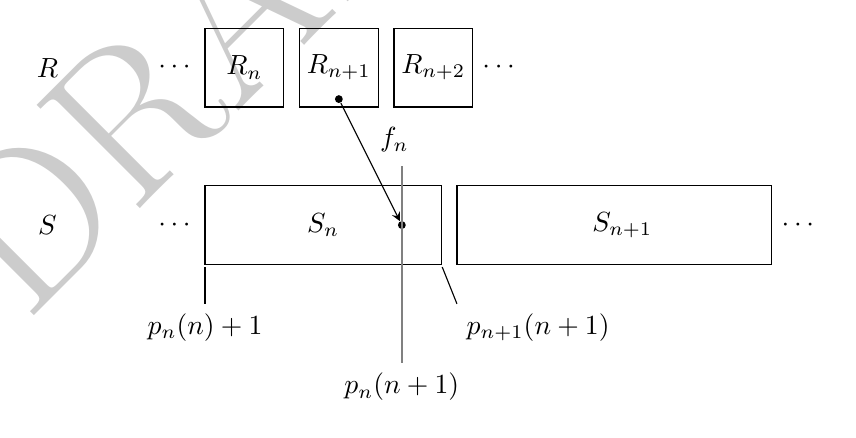
\begin{tikzpicture}[yscale=0.5]
        \begin{scope}[shift={(0, 5)}]
          \node at (0, 1) {$R$};

          %% Rectangles for equivalence classes of $R$.
          \draw (2, 0)
          %% TODO should be a way to use [current node is local] option here...
          ++(0, 1) node[anchor=east] {$\dotsb$} ++(0, -1)
          rectangle ++(1, 2)
          ++(0.2, -2)
          rectangle ++(1, 2)
          ++(0.2, -2)
          rectangle ++(1, 2)
          ++(0, -1)
          node[anchor=west] {$\dotsb$}
          ;

          %% Labels for each equivalence class of $R$.
          \path
          (2.5, 1) node {$R_n$}
          ++(1.2, 0) node {$R_{n + 1}$}
          ++(1.2, 0) node {$R_{n + 2}$}
          ;
        \end{scope}

        %% Arrow from top to bottom showing image under $f_n$.
        \begin{scope}[shift={(0, 1)}]
          \draw
          (4.5, 1) node[shape=circle, fill=black, inner sep=1pt] (source) {}
          ++(-0.8, 3.2) node[shape=circle, fill=black, inner sep=1pt] (target) {};
          \path[<-, >=stealth] (source) edge node[anchor=south west] {$f_n$} (target);
        \end{scope}

        \begin{scope}[shift={(0, 1)}]
          \node at (0, 1) {$S$};

          %% Rectangles for equivalence classes of $S$.
          \draw (2, 0)
          %% TODO should be a way to use [current node is local] option here...
          ++(0, 1) node[anchor=east] {$\dotsb$} ++(0, -1)
          rectangle ++(3, 2)
          ++(0.2, -2)
          rectangle ++(4, 2)
          ++(0, -1)
          node[anchor=west] {$\dotsb$}
          ;

          %% Labels for each equivalence class of $S$.
          \path
          (3.5, 1) node {$S_n$}
          ++(3.8, 0) node {$S_{n + 1}$}
          ;
        \end{scope}

        %% Labels underneath each $S_i$ showing length bounds.
        \begin{scope}
          \draw[shorten >=1pt]
          (2, 0) node[anchor=north] (pn) {$p_n(n) + 1$}
          -- ++(0, 1);
          \draw[thick, color=gray] (4.5, 3.5)
          -- ++(0, -5)
          node[anchor=north, color=black] (pnplus1) {$p_n(n + 1)$}
          ;
          \draw[shorten >=1pt]
          (5.2, 0) node[anchor=north west, color=black] (pnplus1nplus1) {$p_{n + 1}(n + 1)$}
          -- ++(-0.2, 1);
          ;
        \end{scope}
      \end{tikzpicture}
    \end{center}
  \end{figure}

  Finally, we show that $R$ and $S$ are in $\NC^1$.
  Deciding whether two strings have the same length is trivial, so $R$ is certainly in $\NC^1$.
  To decide $S$, we compute the index $i$ of the equivalence class $S_i$ containing the string $x$ and the index $j$ of the equivalence class $S_j$ containing the string $y$, then compare them for equality.
  Computing the index $i$ of the equivalence class of a string $x$ of length $n$ can be performed as follows.
  First, compute in parallel the values $p_1(1), \dotsc, p_{n + 1}(n + 1)$.
  Since each $p_i$ is increasing, $n$ is definitely smaller than $p_{n + 1}(n + 1)$.
  Computing the exponentiation of $O(n)$ pairs of strings of length $O(n)$ each can be performed by a $\TC^0$ circuit, and $\TC^0 \subseteq \NC^1$.
  Next, for each $i \in \{1, \dotsc, n\}$ in parallel, decide if $p_i(i) + 1 \leq n \leq p_{i + 1}(i + 1)$, thereby determining whether the input is in $S_i$.
  These comparisons can be performed by an $\NC^1$ circuit.
  Finally, use $O(\log n)$ single-bit multiplexers in parallel to output the index (in binary) of the sole equivalence class $S_i$ containing $x$.
  A single-bit multiplexer for $O(\log n)$ input bits can be implemented by a circuit of size $O(\log n)$ and depth $O(\log \log n)$ \autocite[Lemma~2.5.5]{savage98}, so this phase of the computation can be performed by an $\NC^1$ circuit.
  Computing the indices $i$ and $j$ for the two input strings can be performed in parallel, and the final comparison for equality of $i$ and $j$ adds only $O(\log n)$ depth to the circuit.
  Therefore $S \in \NC^1$.
\end{proof}

%% generalcompleteness.tex - completeness under kernel reductions
%%
%% Copyright 2010, 2011, 2012, 2014 Jeffrey Finkelstein.
%%
%% This LaTeX markup document is made available under the terms of the Creative
%% Commons Attribution-ShareAlike 4.0 International License,
%% https://creativecommons.org/licenses/by-sa/4.0/.
\section{Conditions for complete problems under polynomial time kernel reductions}
\label{sec:generalcompleteness}

In this section we use the techniques of \autocite[Theorem~8.7]{bcffm} to present a general theorem which provides equivalence relations which are hard for a number of interesting complexity classes under polynomial time kernel reductions.
We need one additional definition here.
If $\mathcal{C}$ is a complexity class then the class $\forall\mathcal{C}$ is the set of languages $A$ such that there exists a language $B\in\mathcal{C}$ and a polynomial $p$ satisfying $x\in A$ if and only if $\forall w\in\Sigma^{\leq p(|x|)} \pair{x}{w}\in B$.
$\forall\mathcal{C}$ is called the \defn{closure of $\mathcal{C}$ under polynomially bounded universal quantification}.

\begin{theorem}\label{thm:generalcompleteness}
  Let $\mathcal{C}$ be a subset of $\PSPACE$ which contains the problem of deciding whether two strings are equal.
  Then there exists an equivalence relation in $\CRAZYEq$ which is hard for $\CEq$ under $\kr$ reductions.
\end{theorem}

Before proving this theorem, we will provide some immediate corollaries of this general result.

\begin{corollary}
  If $\mathcal{C}$ is a subset of $\PSPACE$ and $\mathcal{C}=\CRAZY$, then $\CEq$ has a complete problem under $\kr$ reductions.
\end{corollary}

\begin{corollary}\label{cor:hardproblems}
  Under polynomial time kernel reductions,
  \begin{enumerate}
  %\item $\EXPEq$ has a complete problem
  \item $\PSPACEEq$ has a complete problem
  \item $\PKPEq$ contains a problem that is hard for $\DKPEq$, for all $k \geq 1$
  %\item\label{itm:hardforsigma} $\PKPOPEq$ contains a problem which is hard for $\SKPEq$, for all $k\geq 0$
  %\item $\PKPOPEq$ contains a problem which is hard for $\PKPEq$, for all $k\geq 0$
  %\item $\coNPEq$ contains a problem which is hard for $\PEq$
  \end{enumerate}
\end{corollary}
\begin{proof}\mbox{}
  \begin{enumerate}
  %\item $\EXP$ is closed under complement (because it is a deterministic complexity class) and polynomially bounded universal quantification (because we can simulate the universal guess deterministically in exponential time).
  \item $\PSPACE$ is closed under complement (because it is a deterministic complexity class) and polynomially bounded universal quantification (because we can simulate the universal guess deterministically in polynomial space).
  \item
    First, $(\forall(\DKP \cup \mathsf{co}\DKP))\mathsf{Eq} = (\forall \DKP)\mathsf{Eq}$, since $\DKP$ is closed under complement.  % \autocite[Proposition~8.4 (a)]{bdg95}
    Next, $(\forall \DKP)\mathsf{Eq} = \PKPEq$, since $\forall \DKP = \PKP$.  % \autocite[Proposition~8.3 (g)]{bdg95}
    Now if we choose $\mathcal{C} = \DKP$ in \autoref{thm:generalcompleteness}, then $\PKPEq$ has a problem that is hard for $\DKPEq$ under $\kr$ reductions.
    \qedhere
  %\item If $\mathcal{C}=\SKP$, then the $\kr$-hard problem is in $(\forall(\SKP\cup\mathsf{co}\SKP))\mathsf{Eq}=(\forall(\SKP\cup\PKP))\mathsf{Eq}=\PKPOPEq$.
  %\item Same as the previous justification, but starting with $\mathcal{C}=\PKP$.\qedhere
%  \item Same as the previous justification, but starting with $\mathcal{C}=\P$.
  \end{enumerate}
\end{proof}

More specifically, this means that $\coNPEq$ (which equals $\POPEq$) has a problem which is $\kr$-hard for $\PEq$ (which equals $\DOPEq$).
This leads to \autocite[Theorem~8.7, part~1]{bcffm}, which is restated here.

\begin{corollary}[{\autocite[Theorem~8.7, part~1]{bcffm}}]
  If $\NP = \coNP$ then $\NPEq$ has a complete problem under polynomial time kernel reductions.
\end{corollary}
\begin{proof}
  If $\NP = \coNP$, then the polynomial hierarchy collapses to $\POP$, and specifically $\PTP = \DTP = \POP = \coNP = \NP$.
  From \autoref{cor:hardproblems} we conclude that $\NPEq$ has a $\kr$-hard problem for $\NPEq$.
  Such a problem is by definition $\NPEq$-complete.
\end{proof}

We now return to the proof of \autoref{thm:generalcompleteness} by first providing some motivating ideas.
Recall the canonical complete problem (sometimes called the ``universal'' problem) for $\NP$ (and indeed for various other complexity classes):
\begin{displaymath}
  K = \lb\triple{M}{x}{1^t} \st M\plain{accepts} x \plain{within} t \textnormal{ steps}\rb
\end{displaymath}
The idea of this proof is to adapt this into an equivalence relation $R_K$ consisting of pairs of triples of the form $\pair{\triple{M}{x}{1^{t_x}}}{\triple{M}{y}{1^{t_y}}}$, where $M$ accepts $\pair{x}{y}$, as in the reduction from an arbitrary $\NP$ language to $K$.
The problem we encounter here is that $R_K$ is not necessarily an equivalence relation.
Consider, for example, transitivity, which must be satisfied for all possible pairs of the form $\triple{M}{w}{1^{t_w}}$.
For \emph{arbitrary machines} $M$, just because $M$ accepts $\pair{x}{y}$ and $\pair{y}{z}$ does not necessarily mean that $M$ accepts $\pair{x}{z}$.
The solution is to encode into $R_K$ the requirement that the language which $M$ accepts, $L(M)$, is itself an equivalence relation.
The three properties required of $R_K$ then follow from the properties of $L(M)$.
%
%As a technical consideration for this proof, we point out languages in $\PSPACE$ may be decided by alternating Turing machines which run in polynomial time, so it is permissible to consider polynomially clocked Turing machines.
%
\begin{proof}[Proof of \autoref{thm:generalcompleteness}]
  First we will define a helper algorithm which decides whether a given machine accepts an equivalence relation on strings up to a given length.
  Define the algorithm $A$ as follows on input $\pair{M}{n}$, where $M$ is a polynomially clocked Turing machine of type $\mathcal{C}$ and $n\in\mathbb{N}$:
  \begin{enumerate}
  \item universally guess $a,b,$ and $c\in\Sigma^{\leq n}$
  \item simulate $M$ on $\pair{a}{a}$; if it rejects, reject
  \item simulate $M$ on $\pair{a}{b}$, then on $\pair{b}{a}$; if the former accepts and the latter rejects, reject
  \item simulate $M$ on $\pair{a}{b}$, then on $\pair{b}{c}$, then on $\pair{a}{c}$; if the first two accept and the last one rejects, reject
  \item if execution reaches this point, accept
  \end{enumerate}
  These simulations check that $L(M)$ satisfies reflexivity, symmetry, and transitivity on strings of length at most $n$.
  If $A$ accepts, then the three properties are satisfied, and if it rejects then one of the three properties is violated.
  Since $M$ is a machine of type $\mathcal{C}$, checking if $M$ accepts on some input and if $M$ rejects on some input is in $\mathcal{C}\cup\mathsf{co}\mathcal{C}$.
  The universal guesses of $a,b,$ and $c$ (of length at most $n$) followed by checks of whether the six simulations of $M$ accept or reject place $L(A)$ in the class $\CRAZY$.
  If $p$ is the polynomial which bounds the running time of $M$, then the running time of this algorithm is $6p\left(\left|\pair{1^n}{1^n}\right|\right)+c$, where $c$ is a constant which represents the time needed to account for the implementation of $A$ (the control of the simulations of $M$, performing logical conjunctions, etc.).
  Hence the running time of $A$ is polynomial in $n$.

  Now we can define the set $R_K$ by
  \begin{align*}
    R_K = {} & \lb\pair{u}{v} \st u=v\rb \\
    & \cup \lb\pair{\triple{M}{x}{1^{t_x}}}{\triple{M}{y}{1^{t_y}}} \st \textnormal{1 through 4 below are satisfied}\rb
  \end{align*}
  where the conditions are
  \begin{enumerate}
  \item\label{itm:machine} $M$ is a polynomially clocked Turing machine of type $\mathcal{C}$
  \item\label{itm:emx} $A$ accepts $\pair{M}{|x|}$ within $t_x$ steps
  \item\label{itm:emy} $A$ accepts $\pair{M}{|y|}$ within $t_y$ steps
  \item\label{itm:accepts} $M$ accepts $\pair{x}{y}$
  \end{enumerate}
  We claim that $R_K$ is in $\CRAZYEq$ and $\CEq$-hard.

  First we show that $R_K\in\CRAZY$.
  By the argument above, $A$ is a $\CRAZY$ algorithm.
  %Since $M$ is a polynomially clocked $\mathcal{C}$ machine by \autoref{itm:machine}, then the simulation of $M$ on $\pair{x}{y}$ in \autoref{itm:accepts} can be performed by a $\mathcal{C}$ algorithm.
  Assuming without loss of generality that $|x|\geq |y|$, if $A$ accepts $\pair{M}{|x|}$ within $t_x$ steps then we know that there is a polynomial time bound on the running time of $M$ on input $\pair{x}{y}$, so simulating it is certainly in $\CRAZY$.
  Finally, testing for equality is in $\mathcal{C}$ by hypothesis so deciding $R_K$ overall can be performed by a $\CRAZY$ algorithm.

  Next we show that $R_K$ is an equivalence relation.
  Reflexivity follows from the reflexivity of the equality relation.
  For symmetry, suppose $\pair{\triple{M}{x}{1^{t_x}}}{\triple{M}{y}{1^{t_y}}}\in R_K$.
  Since \autoref{itm:emx} and \autoref{itm:emy} are true by hypothesis, we know that symmetry on strings of length at most $\max(|x|, |y|)$ in $L(M)$ is satisfied, and that includes the strings $x$ and $y$.
  So since $M$ accepts $\pair{x}{y}$ it must follow that $M$ accepts $\pair{y}{x}$.
  Furthermore, \autoref{itm:machine}, \autoref{itm:emx}, and \autoref{itm:emy} are the same up to symmetry of $x$ and $y$, so we have $\pair{\triple{M}{y}{1^{t_y}}}{\triple{M}{x}{1^{t_x}}}\in R_K$.
  For transitivity, suppose that both $\pair{\triple{M}{x}{1^{t_x}}}{\triple{M}{y}{1^{t_y}}}\in R_K$ and $\pair{\triple{M}{y}{1^{t_y}}}{\triple{M}{z}{1^{t_z}}}\in R_K$.
  Since transitivity is true on strings of length at most $\max(|x|, |y|, |z|)$ by the transitivity propositions checked by \autoref{itm:emx} and \autoref{itm:emy}, and since $M$ accepts both $\pair{x}{y}$ and $\pair{y}{z}$ by hypothesis, it must follow that $M$ accepts $\pair{x}{z}$.
  Again the conditions in \autoref{itm:machine}, \autoref{itm:emx}, and \autoref{itm:emy} are the same.
  We have shown that $R_K$ is reflexive, symmetric, and transitive, so it is an equivalence relation.
  At this point, we have proven that $R_K\in\CRAZYEq$.

  Now we need to show that $R_K$ is $\CEq$-hard.
  Let $S\in\CEq$.
  Suppose $M$ is the polynomially clocked $\mathcal{C}$ machine which decides $S$, and $p$ is the polynomial which bounds the running time of $M$.
  Then the kernel reduction from $S$ to $R_K$ is $w\mapsto\triple{M}{w}{1^{6p(|\pair{w}{w}|)+c}}$, where $p$ and $c$ are the polynomial and constant described in the first paragraph of this proof.
  Call this reduction $f$.
  The reduction is obviously computable in time polynomial in $|w|$.
  It remains to show that this reduction is correct.

  Suppose $\pair{x}{y}\in S$.
  Now $f(x)=\triple{M}{x}{1^{6p(|\pair{x}{x}|)+c}}$ and $f(y)=\triple{M}{y}{1^{6p(|\pair{y}{y}|)+c}}$.
  \autoref{itm:machine} is true by construction, and \autoref{itm:accepts} is true since $M$ is the machine which decides $S$.
  Assume \autoref{itm:emx} is false.
  Then $M$ does not accept an equivalence relation on strings of length at most $|x|$.
  This is a contradiction, since $M$ decides $S$, an equivalence relation, by hypothesis.
  Therefore \autoref{itm:emx} must be satisfied.
  The same argument applies to \autoref{itm:emy}.
  Hence $\pair{f(x)}{f(y)}\in R_K$.

  If $\pair{x}{y}\notin S$ then $M$ does not accept $\pair{x}{y}$, since otherwise $\pair{x}{y}$ would be a member of $S$.
  Hence $\pair{x}{y}\notin R_K$.
  Therefore we have shown that $R_K$ is $\CEq$-hard.
\end{proof}

\begin{openproblem}
  Is there a more general characterization of complexity classes which have a $\kr$-hard problem?
\end{openproblem}

\begin{openproblem}
  Under what conditions does a complexity class have a complete problem?
  Can we adapt this idea to create a complete problem for $\PEq$ or $\NPEq$?
\end{openproblem}

\begin{openproblem}
  Can this theorem be used to construct $\krnt$-hard problems for smaller complexity classes like $\NLEq$ under the appropriate time-bounded reduction?
  Larger classes such as $\EXPEq$?
\end{openproblem}

\begin{openproblem}
  To what other equivalence relations does our $\kr$-hard problem reduce?
  Are there ``natural'' $\kr$-hard problems in complexity classes which satisfy the conditions in \autoref{thm:generalcompleteness}?
\end{openproblem}

%% As an additional corollary, we show that the equivalence relation $R_K$ is necessarily hard given a known hard equivalence relation under $\kr$ reductions.

%% \begin{corollary}
%%   Let $\mathcal{C}_1$ be a complexity class and $\mathcal{C}_2$ be a subset of $\PSPACE$ which contains the problem of deciding whether two strings are equal.
%%   If there exists an equivalence relation $S$ in $\CTEq$ which is hard for $\COEq$ under $\kr$ reductions, then there is an equivalence relation in $\CRAZIEREq$ which is hard for $\COEq$ under $\kr$ reductions.
%% \end{corollary}
%% \begin{proof}
%%   $S\kr R_K$ by the reduction described in the proof of \autoref{thm:generalcompleteness}.
%%   A similar analysis shows that $R_K\in\CRAZIEREq$.
%%   Since $S$ is hard for $\COEq$ and polynomial time kernel reductions compose, $R_K$ is also hard for $\COEq$.
%% \end{proof}

%% This last question leads us to briefly note that equivalence of true quantified boolean formulas is a \PSPACE-complete problem; perhaps it is also a \PSPACEEq-complete problem.
%% \begin{proposition}
%%   Define $\QBFEq$ by
%%   \begin{displaymath}
%%     \QBFEq = \{\pair{\phi}{\psi} | \phi \iff \psi\},
%%   \end{displaymath}
%%   where $\phi$ and $\psi$ are fully quantified boolean formulae.
%%   Then $\QBFEq$ is \PSPACE-complete.
%% \end{proposition}
%% \begin{proof}
%%   Suppose $\phi$ denotes $\overline{Q}\tau$, where $\overline{Q}$ represents the sequence of quantified variables and $\tau$ is the boolean formula over those variables.
%%   Then the many-one reduction from $\QBF$ is $\phi\mapsto\pair{\phi}{\exists z\colon\overline{Q}(\tau\land z)}$, where $z$ is a variable not already in $\phi$.
%%   This reduction can obviously be computed in time polynomial in the length of the input, $\phi$.
%%   If $\phi$ is not satisfiable, then no assignment of $z$ makes $\overline{Q}(\tau\land z)$ satisfiable, because $\tau$ will always be false.
%%   Hence $\exists z\colon\overline{Q}(\tau\land z)$ must be false.
%%   If $\phi$ is satisfiable, then choosing $z$ to be true makes $\overline{Q}(\tau\land z)$ true.
%%   Thus $\phi$ is satisfiable if and only if $\exists z\colon\overline{Q}(\tau\land z)$ is satisfiable, so $\QBF\mor\QBFEq$.
%%   Since $\QBFEq$ is clearly decidable in $\PSPACE$, we conclude that $\QBFEq$ is \PSPACE-complete.
%% \end{proof}

%% npeqcompleteness.tex - completeness in NP equivalence classes
%%
%% Copyright 2010, 2011, 2012, 2014, 2015 Jeffrey Finkelstein.
%%
%% This LaTeX markup document is made available under the terms of the Creative
%% Commons Attribution-ShareAlike 4.0 International License,
%% https://creativecommons.org/licenses/by-sa/4.0/.
\section
    [Relationship between completeness under kernel and many-one reductions]
    {Relationship between completeness \\ under kernel and many-one reductions}
\label{sec:npeqcompleteness}
% Foreword
%
% context (focus on anyone) why now? - current situation, and why the need is so important
A kernel reduction implies a many-one reduction, but does completeness under kernel reductions imply completeness under many-one reductions?
% need (focus on readers) why you? - why this is relevant to the reader, and why something needed to be done
Since polynomial-time kernel reductions are different from polynomial-time many-one reductions (\autoref{thm:different}), completeness in classes of equivalence problems may differ under these reductions as well.
% task (focus on author) why me? - what was undertaken to address the need
We determine the conditions under which completeness under kernel reductions implies completeness under many-one reductions.
% object (focus on document) why this document - what the document covers
%This section presents some information about the relationship between these two types of reductions.

% Summary
%
% findings (focus on author) what? - what the work revealed when performing the task
We find that completeness under many-one reductions follows as a straightforward consequence of completeness under kernel reductions as long as the relevant complexity class admits a complete problem under many-one reductions.
We also show that the kernel reduction is essentially too weak to allow for completeness under injective (that is, ``one-to-one'') reductions, for combinatorial reasons similar to those in \autoref{sec:limitations}.
Though we prove these results for $\NPEq$, they generalize in a natural way to any ``well-behaved'' complexity class (basically, any class containing a complete problem under many-one reductions).
% conclusion (focus on readers) so what? - what the findings mean for the audience
These results are more indication that when comparing the relative difficulty of equivalence problems, one should attempt to construct a kernel reduction instead of a many-one reduction.
% perspective (focus on anyone) what now? - what should be done next
The potential lack of a complete problem under injective kernel reductions suggests that a conjecture analagous to the Berman--Hartmanis conjecture, which states that all $\NP$-complete problems are isomorphic with respect to many-one reductions, may be false in $\NPEq$.

One can infer the existence of $\NP$-complete equivalence relations from the relation suggested in \autocite[Section~6.2]{fg11},
\begin{equation*}
  \{\pair{0\phi}{1\phi} \, | \, \phi \in \textsc{Satisfiability}\}.
\end{equation*}
(This relation is not itself an equivalence relation, but can be modified to guarantee the three necessary properties.)
Using this idea, we provide a strategy for constructing a more natural $\NP$-complete equivalence relation from an equivalence relation in $\NP$ and an arbitrary $\NP$-complete property.

Let \textsc{GI} denote the equivalence relation consisting of all pairs of isomorphic graphs.
A property, that is, a Boolean function, $\Pi$ is an \defn{$\NP$-complete property} if $L_\Pi$, the set of all strings for which $\Pi$ is true, is $\NP$-complete.
If, furthermore, the property satisfies $\pair{x}{y} \in R$ implies $\Pi(x) = \Pi(y)$ where $R$ is an equivalence relation, $\Pi$ is called a \emph{property on $R$}.
For example, Hamiltonicity, the property of having a cycle that includes each vertex, is an $\NP$-complete property on \textsc{GI}.

\begin{theorem}\label{thm:npceqrel}
  If $\Pi$ is an \NP-complete property on \textsc{GI}, then the equivalence relation $A$ defined by
  \begin{equation*}
    A = \left\{ \pair{G}{H} \, \middle| \, \pair{G}{H} \in \textsc{GI} \text{ or } (G \in L_\Pi \text{ and } H \in L_\Pi) \right\}
  \end{equation*}
  is an \NP-complete equivalence relation.
\end{theorem}
\begin{proof}
  It is straightforward to prove that $A$ is an equivalence relation, so it remains to show that it is $\NP$-complete.
  The language $A$ is in $\NP$ because both $R$ and $L_\Pi$ are in $\NP$ by hypothesis.
  Thus we need only show that $A$ is $\NP$-hard.

  Let $H$ be a graph satisfying $\Pi$; such a graph must exist because $\Pi$ is $\NP$-complete and therefore there must be at least one graph that satisfies $\Pi$ and at least one that does not (otherwise no many-one reduction to $L_\Pi$ could exist).
  The reduction proving that $A$ is $\NP$-complete is from $L_\Pi$, and the mapping is given by $G \mapsto \pair{G}{H}$.
  This function is computable in linear time; the size of $H$ is constant with respect to the size of $G$.

  Now we show that $G \in L_\Pi$ if and only if $\pair{G}{H} \in A$, for any graph $G$.
  If $G \in L_\Pi$, then $G \in L_\Pi$ and $H \in L_\Pi$, so $\pair{G}{H} \in A$.
  If $\pair{G}{H} \in A$, then either $G \in L_\Pi$ and $H \in L_\Pi$, in which case $G \in L_\Pi$, or $G$ is isomorphic to $H$, in which case $G$ is in $L_\Pi$ because $H$ is.
  In either case $G \in L_\Pi$.
  We conclude that $L_\Pi \mor A$, and so $A$ is an $\NP$-complete equivalence relation.
\end{proof}

\begin{example}\label{ex:npceqrel}
  The language
  \begin{equation*}
    \left\{ \pair{G}{H} \, \middle| \, \pair{G}{H} \in \textsc{GI} \text{ or } G \text{ and } H \text{ have a Hamiltonian cycle}  \right\}
  \end{equation*}
  is an \NP-complete equivalence relation.
\end{example}

There are other ways of constructing a natural $\NP$-complete equivalence relation.
For example, there is a finitely presented group whose word problem is $\NP$-complete \autocite[Corollary~1.1]{sbr02}, and the word problem is already an equivalence relation.
This may be considered ``more natural'' because it does not involve the disjunction of two distinct computational problems, though it lacks the simplicity of our approach.

\begin{example}
  As stated briefly above, \autoref{thm:npceqrel} can be generalized to isomorphism of structures other than graphs and/or larger complexity classes.
  For example, replacing \textsc{GI} with \textsc{FI}, the Boolean formula isomorphism problem, and an $\NP$-complete property on \textsc{GI} with a $\SigmaTwoP$-complete property on \textsc{FI} yields a $\SigmaTwoP$-complete equivalence relation.
\end{example}

\begin{corollary}
  If $R$ is $\NPEq$-complete, then $R$ is $\NP$-complete.
\end{corollary}
\begin{proof}
  This follows immediately from the existence of an $\NP$-complete equivalence relation, as in \autoref{ex:npceqrel}, and the fact that a kernel reduction implies a many-one reduction.
\end{proof}

This corollary provides a clearer proof of \autocite[Proposition~8.1]{bcffm}.

\begin{corollary}[{\autocite[Proposition~8.1]{bcffm}}]
  If \textsc{GI} is \NPEq-complete then the polynomial hierarchy collapses to the second level, that is, $\PH = \STP$.
\end{corollary}
\begin{proof}
  By the previous corollary, if \textsc{GI} is $\NPEq$-complete, then it is $\NP$-complete, which implies the stated collapse (see \autocite{schoning87}).
\end{proof}

\autoref{thm:npceqrel} also provides a simple method for proving the equivalence of $\P = \NP$ and $\PEq = \NPEq$.

\begin{theorem}\label{thm:pnppeqnpeq}
  $\P = \NP$ if and only if $\PEq = \NPEq$.
\end{theorem}
\begin{proof}
  If $\P = \NP$, then $\PEq = \NPEq$ by their definitions.
  Suppose now that $\PEq = \NPEq$.
  Let $A$ denote the $\NP$-complete equivalence relation defined in \autoref{ex:npceqrel}.
  Since $A \in \NPEq$ and $\PEq = \NPEq$ by hypothesis, $A \in \PEq$, and hence $A \in \P$.
  Since $\P$ is closed under $\mor$ reductions, any $\NP$-complete problem in $\P$ implies $\P = \NP$.
\end{proof}

As stated in \autoref{sec:generalcompleteness}, we do not know whether an $\NPEq$-complete problem exists.
In the following theorem we describe an equivalence relation that, if it were $\NPEq$-complete, would prove that injective kernel reductions are strictly weaker than general kernel reductions.
This is interesting because it again demonstrates that the number and size of equivalence classes is important when considering the (im)possibility of polynomial-time kernel reductions between equivalence relations.
In the following theorem, if an equivalence relation is ``complete under $\kri$ reductions in $\NPEq$'' we mean that every equivalence relation in $\NPEq$ reduces to it by a polynomial-time computable kernel reduction which is also injective (that is, ``one-to-one'').

\begin{theorem}\label{thm:inj}
  Let $\Pi$ be a property on \textsc{GI}.
  %% If for each natural number $n$ there is a graph $G$ of size $n$ such that $\Pi(G) = 1$, and 
  If the equivalence relation $A$ defined by
  \begin{equation*}
    A = \left\{ \pair{G}{H} \, \middle| \, \pair{G}{H} \in \textsc{GI} \text{ or } (G \in L_\Pi \text{ and } H \in L_\Pi \text{ and } |G| = |H|) \right\}
  \end{equation*}
  is complete for $\NPEq$ under $\kr$ reductions, then $A$ is not complete under $\kri$ reductions.
\end{theorem}

The only difference between the equivalence relation $A$ defined here and the one defined in \autoref{thm:npceqrel} is the requirement that $|G| = |H|$.
This means that although the number of equivalence classes in $A$ is infinite (at least one for each size), each of those equivalence classes is itself finite.
In contrast, consider the equivalence relation $S$ defined by
\begin{equation*}\label{eq:ones}
  S = \left\{ \pair{x}{y} \, \middle| \, x \text{ and } y \text{ have the same number of } 1 \text{s} \right\}.
\end{equation*}
The equivalence relation $S$ has an infinite number of equivalence classes: $[1]$, $[11]$, $[111]$, etc.
Each equivalence class is itself infinite as well: for each $w \in \Sigma^*$, the equivalence class $[w]$ contains $w$, $0w$, $00w$, etc.

\begin{proof}[Proof of \autoref{thm:inj}]
  Let $S$ be the equivalence relation defined in the preceding paragraph.
  The language $S$ is decidable in linear time by a deterministic Turing machine, hence it is in $\NP$.
  Since $A$ is $\NPEq$-complete by hypothesis, $S \kr A$.
  Thus there is a polynomial-time computable function $f$ such that $\pair{x}{y} \in S$ if and only if $\pair{f(x)}{f(y)} \in A$.

  By the discussion preceding this theorem, $[w]_S$ is infinite and $[f(w)]_A$ is finite.
  Since a kernel reduction must preserve equivalence classes, $f([w]_S) \subseteq [f(w)]_A$.
  Consider $f|_{[w]_S}$, that is, $f$ restricted to the domain $[w]_S$.
  Then $f|_{[w]_S}$ is a mapping from the infinite set $[w]_S$ to the finite set $[f(w)]_A$.
  By the pigeonhole principle, $f|_{[w]_S}$ is not injective.
  Hence the unrestricted reduction $f$ is not injective, and therefore $A$ is not $\kri$-complete in $\NPEq$.
\end{proof}

%%%%
%% intermediary.tex
%%
%% Copyright 2011 Jeffrey Finkelstein
%%
%% Except where otherwise noted, this work is made available under the terms of
%% the Creative Commons Attribution-ShareAlike 3.0 license,
%% http://creativecommons.org/licenses/by-sa/3.0/.
%%
%% You are free:
%%    * to Share — to copy, distribute and transmit the work
%%    * to Remix — to adapt the work
%% Under the following conditions:
%%    * Attribution — You must attribute the work in the manner specified by
%%    the author or licensor (but not in any way that suggests that they
%%    endorse you or your use of the work).
%%    * Share Alike — If you alter, transform, or build upon this work, you may
%%    distribute the resulting work only under the same, similar or a 
%%    compatible license.
%%    * For any reuse or distribution, you must make clear to others the 
%%    license terms of this work. The best way to do this is with a link to the
%%    web page http://creativecommons.org/licenses/by-sa/3.0/.
%%    * Any of the above conditions can be waived if you get permission from
%%    the copyright holder.
%%    * Nothing in this license impairs or restricts the author's moral rights.
%%%%
\section{Existence of intermediary problems}

We will denote by $\NPEqC$ the set of equivalence relations which are $\kr$-complete for \NPEq.

The main result of this section is as follows.
\begin{reptheorem}{thm:intermediary}
  \printintermediarytheorem
\end{reptheorem}
To show this, we will adapt a proof of Ladner's original theorem\cite{ladner} showing that if $\P\neq\NP$ then there exist problems in $\NP$ which are neither in $\P$ nor \NP-complete.
The proof we follow can be found in \cite{bdg95}, which is an adaptation of Sch\"{o}ning's proof of the ``uniform diagonalization theorem''\cite{schoning}, which is itself a generalization of Ladner's original method.

First we need to provide some technical definitions and machinery.

\begin{definition}
  A class of languages $\mathcal{C}$ is \defn{closed under finite variations} if and only if $A\in \mathcal{C}$ and $A\symdiff B$ (the symmetric difference of $A$ and $B$) is finite implies $B\in \mathcal{C}$ for all $B$.
\end{definition}

\begin{definition}
  Given an alphabet $\Sigma$ with at least two different symbols, say $0$ and $1$, the \defn{kernel join} of two equivalence relations $R$ and $S$ over $\Sigma^*$ is $R\kj S=\{\pair{x0}{y0}|\pair{x}{y}\in R\}\cup\{\pair{x1}{y1}|\pair{x}{y}\in S\}$.
\end{definition}

\begin{lemma}\label{lem:join}
  If $R$ and $S$ are equivalence relations on $\Sigma^*$, then $R\kj S$ is an equivalence relation (on $\Sigma^*\backslash\{\lambda\}$).
\end{lemma}
\begin{proof}
  Let $x$, $y$ and $z$ be non-empty strings in $\Sigma^*$.
  
  Since $x$ is non-empty, $x=x'0$ or $x=x'1$.
  Since $R$ is reflexive, $\pair{x'}{x'}\in R$.
  Hence $\pair{x}{x}\in R\kj S$.
  Therefore $R\kj S$ is reflexive.
  
  Suppose $\pair{x}{y}\in R\kj S$.
  Then either $x=x'0$, $y=y'0$ and $\pair{x'}{y'}\in R$ or $x=x'1$, $y=y'1$ and $\pair{x'}{y'}\in S$.
  In either case, symmetry follows from the symmetry of $R$ or $S$.

  Suppose $\pair{x}{y}$ and $\pair{y}{z}$ are both in $R\kj S$.
  In the case that $x=x'0$, $y=y'0$ and $\pair{x'}{y'}\in R$, and that $z=z'0$ and $\pair{y'}{z'}\in R$, then by the transitivity of $R$, $\pair{x'}{z'}\in R$, so $\pair{x}{z}\in R\kj S$.
  The argument is similar in the case that $x=x'1$, $y=y'1$ and $z=z'1$.
  It is a contradiction for the other two cases to exist, since $y$ cannot be equal to both $y'0$ and $y'1$.

  Since $R\kj S$ is reflexive, symmetric and transitive, $R\kj S$ is an equivalence relation.
\end{proof}

\begin{proposition}\label{prop:symdiff}
  Symmetric difference of equivalence relations preserves symmetry.
\end{proposition}
\begin{proof}
  Let $R$ and $S$ be equivalence relations.
  Let $(x,y)\in(R\symdiff S)$.
  In the case that $(x,y)\in R$ and $(x,y)\notin S$, then $(y,x)\in R$.
  If $(y,x)$ were in $S$, then $(x,y)$ would also be in $S$, by symmetry, but this is a contradiction.
  Hence $(y,x)\in R$ and $(y,x)\notin S$.
  The argument for the other case is symmetric.
  Therefore $(x,y)\in(R\symdiff S)\implies (y,x)\in(R\symdiff S)$.
\end{proof}

\begin{definition}
  Let $r\colon\mathbb{N}\to\mathbb{N}$ be a computable function such that $r(m)>m$ for all $m$.
  Define the set $G[r]$ as
  \begin{displaymath}
    G[r]=\{x\in\Sigma^*|r^n(0)\leq|x|<r^{n+1}(0) \plain{for some even} n\}
  \end{displaymath}
  where $r^n(m)$ denotes the $n$-fold application of $r$ to $m$:
  \begin{displaymath}
    \overbrace{r\circ r\circ r\circ\cdots\circ r}^{n \plain{times}}(m)
  \end{displaymath}
  $G[r]$ is called the \defn{gap language} generated by $r$.
\end{definition}

\begin{lemma}\label{lem:gap_p}
  If $r$ is time constructible, then $G[r]\in\P$.
\end{lemma}
\begin{proof}
  Proof omitted.
\end{proof}

We will denote the Cartesian product $G[r]\times G[r]$ by the slightly more succinct ${G[r]}^2$, and $\overline{G[r]}\times\overline{G[r]}$ by $\overline{G[r]}^2$.
Elements of ${G[r]}^2$ are pairs of strings whose lengths are in the ``even gaps'' of $r$, while elements of $\overline{G[r]}^2$ are pairs of strings whose lengths are in the ``odd gaps'' of $r$.

\begin{lemma}
  ${G[r]}^2$ and $\overline{G[r]}^2$ are \defn{partial equivalence relations} (that is, they are symmetric and transitive).
\end{lemma}
\begin{proof}
  We will prove the theorem for ${G[r]}^2$; a symmetric argument proves the theorem for $\overline{G[r]}^2$.

  Let $x,y\in\Sigma^*$.
  Suppose $\pair{x}{y}\in {G[r]}^2$, so the lengths of $x$ and $y$ are both in an even gap of $r$.
  Then $\pair{y}{x}\in{G[r]}^2$, so ${G[r]}^2$ is symmetric.
  Now let $z\in\Sigma^*$ and suppose also that $\pair{y}{z}\in {G[r]}^2$.
  Then $y$ and $z$ are both in an even gap of $r$, so $x$, $y$ and $z$ are all in some even gap of $r$, and hence $\pair{x}{z}\in {G[r]}^2$.
  Therefore ${G[r]}^2$ is transitive.
\end{proof}

We are now prepared to prove the main technical theorem which will allow us to construct an equivalence relation which is ``between'' two complexity classes.

\begin{theorem}\label{thm:diag}
  Let $R_1$ and $R_2$ be decidable equivalence relations, and let $\mathcal{C}_1$ and $\mathcal{C}_2$ be classes of decidable equivalence relations such that:
  \begin{enumerate}
  \item $R_1\notin\mathcal{C}_1$
  \item $R_2\notin\mathcal{C}_2$
  \item $\mathcal{C}_1$ and $\mathcal{C}_2$ are computably enumerable
  \item $\mathcal{C}_1$ and $\mathcal{C}_2$ are closed under finite variations
  \end{enumerate}
  Then there exists a decidable equivalence relation $R$ such that:
  \begin{enumerate}
  \item $R\notin \mathcal{C}_1$
  \item $R\notin \mathcal{C}_2$
  \item $R\kr R_1\kj R_2$
  \end{enumerate}
\end{theorem}
\begin{proof}
  Let $P_1, P_2, \ldots$ and $Q_1, Q_2, \ldots$ be enumerations of Turing machines deciding the languages in $\mathcal{C}_1$ and $\mathcal{C}_2$ respectively.
  Define the functions
  \begin{eqnarray*}
    r_1(n)=\underset{i\leq n}{max}\{|z_{i,n}|\}+1 & \text{and} &
    r_2(n)=\underset{i\leq n}{max}\{|z'_{i,n}|\}+1
  \end{eqnarray*}
  where $z_{i,n}$ is the smallest word in $\Sigma^*$ such that there exists an $x\in\Sigma^*$, with $n<|x|\leq|z_{i,n}|$, such that $\pair{z_{i,n}}{x}\in(L(P_i)\symdiff R_1)$, and $z'_{i,n}$ is the smallest word in $\Sigma^*$ such that there exists an $x'\in\Sigma^*$, with $n<|x'|\leq|z'_{i,n}|$, such that $\pair{z'_{i,n}}{x'}\in(L(Q_i)\symdiff R_2)$.
  Note that it also suffices to find an $x$ and $x'$ such that $\pair{x}{z_{i,n}}\in(L(P_i)\symdiff R_1)$ and $\pair{x'}{z'_{i,n}}\in(L(Q_i)\symdiff R_2)$, since symmetric difference on equivalence relations preserves symmetry by \autoref{prop:symdiff}.
  The more important requirement is that $|x|\leq|z_{i,n}|$, since we will require below that both $x$ and $z_{i,n}$ are in the same gap of a specific function.

  We claim that $z_{i,n}$ and $z'_{i,n}$ always exist.
  Assume that no such $z_{i,n}$ exists, so there are no words such that there exists an $x\in\Sigma^*$, with $n<|x|\leq|z_{i,n}|$, such that $\pair{z_{i,n}}{x}\in(L(P_i)\symdiff R_1)$.
  Therefore, there are no pairs in $(L(P_i)\symdiff R_1)$ with both elements of length greater than $n$.
  Then there are a finite number of pairs in $L(P_i)\symdiff R_1$, so $R_1$ is a finite variation of $L(P_i)$.
  Since $\mathcal{C}_1$ is closed under finite variations, $R_1\in\mathcal{C}_1$.
  This is a contradiction with the hypothesis that $R_1\notin\mathcal{C}_1$.
  Therefore such a $z_{i,n}$ always exists.
  The argument that $z'_{i,n}$ always exists is similar.

  Since $L(P_i)$ and $L(Q_i)$ are decidable for all $i$, and since $R_1$ and $R_2$ are decidable, so are $L(P_i)\symdiff R_1$ and $L(Q_i)\symdiff R_2$.
  For each $n$, there is a procedure which always halts and which computes $z_{i,n}$.
  A similar procedure computes $z'_{i,n}$.
  The procedure which computes the maximum of a finite set of numbers and which adds one to that value always halts as well, so $r_1$ and $r_2$ are total computable functions.

  Let $r\ge \max(r_1,r_2)$ be a non-decreasing time constructible function, which exists by \autoref{lem:nondec}.
  Now for all $n$ and all $i\leq n$, each element of the pair $\pair{z_{i,n}}{x}$ has length between $n$ and $r_1(n)$, by construction.
  The same is true for $\pair{z'_{i,n}}{x'}$ between $n$ and $r_2(n)$.
  Notice that $\pair{z_{i,n}}{x}$ and $\pair{z'_{i,n}}{x'}$ are ``witnesses'' that $R_1\neq L(P_i)$ and $R_2\neq L(Q_i)$ respectively.
  Hence for all $n$, there are some witnesses between $n$ and $r(n)$ that for all $i\leq n$, $R_1\neq L(P_i)$ and $R_2\neq L(Q_i)$.

  Define $R=({G[r]}^2\cap R_1)\cup(\overline{G[r]}^2\cap R_2)$, so $R$ is equal to pairs of $R_1$ in the ``even gaps'' of r and $R$ is equal to pairs of $R_2$ in the ``odd gaps'' of $r$.
  It remains to show that $R$ is an equivalence relation which satisfies the properties stated in the theorem.

  First we show that $R$ is indeed an equivalence relation.
  Symmetry and transitivity follow from the symmetry and transitivity of $R_1$, $R_2$, ${G[r]}^2$ and $\overline{G[r]}^2$.
  To show reflexivity, suppose $x\in G[r]$.
  Hence $\pair{x}{x}\in {G[r]}^2$.
  Since $R_1$ is an equivalence relation, $\pair{x}{x}\in R_1$.
  Therefore $\pair{x}{x}\in({G[r]}^2\cap R_1)$, so $\pair{x}{x}\in R$.
  The argument for the case that $x\in\overline{G[r]}$ is similar.
  Therefore $R$ is reflexive, symmetric and transitive.

  Next we show that $R\notin\mathcal{C}_1$.
  The argument which proves $R\notin\mathcal{C}_2$ is symmetric.
  Assume $R\in\mathcal{C}_1$ in order to produce a contradiction.
  Then there exists an $i$ such that $R=L(P_i)$.
  Let $m$ be an even integer such that $r^m(0)\geq i$.
  By construction, there exists a pair $\pair{x}{z}$ such that $r^m(0)\leq|x|\leq|z|<r^{m+1}(0)$ and $\pair{x}{z}\in(L(P_i)\symdiff R_1)$.
  Since $m$ is even, $\pair{x}{z}\in {G[r]}^2$.
  Since $R$ is equal to $R_1$ where it coincides with ${G[r]}^2$, then $\pair{x}{z}\in(L(P_i)\symdiff R)$.
  This is a contradiction with the hypothesis that $R=L(P_i)$.
  Therefore $R\notin\mathcal{C}_1$.

  Finally, we show that $R\kr R_1\kj R_2$.
  First, we note that $R_1\kj R_2$ is an equivalence relation by \autoref{lem:join}, so a kernel reduction here is syntactically possible.
  Since $G[r]\in\P$ by \autoref{lem:gap_p}, the function defined by
  \begin{displaymath}
    f(x)=
    \begin{cases}
      x0 & \text{if}\, x\in G[r]\\
      x1 & \text{if}\, x\notin G[r]\\
    \end{cases}
  \end{displaymath}
  is a polynomial time computable function.
  
  To show that $f$ computes the reduction from $R$ to $R_1\kj R_2$ correctly, suppose first that $\pair{x}{y}\in R$, so $\pair{x}{y}$ is in either $({G[r]}^2\cap R_1)$ or $\overline{G[r]}^2\cap R_2)$.
  In the former case, both $x$ and $y$ are in $G[r]$, so $f(x)=x0$ and $f(y)=y0$, and both $x$ and $y$ are in $R_1$, so $\pair{x0}{y0}=\pair{f(x)}{f(y)}\in R_1$.
  The argument for the latter case is symmetric.

  For the converse, suppose $\pair{f(x)}{f(y)}\in R_1\kj R_2$.
  Then $f(x)$ and $f(y)$ either both end with $0$ or both end with $1$.
  In the case that both end with $0$, then there exist some strings $w_x$ and $w_y$ such that $f(x)=w_x0$, $f(y)=w_y0$ and $\pair{w_x}{w_y}\in R_1$.
  By construction of $f$, $w_x$ must equal the input $x$ and $w_y$ must equal the input $y$, so $\pair{x}{y}\in R_1$.
  Also by construction, $f(x)=x0$ if and only if $x\in G[x]$ and $f(y)=y0$ if and only if $y\in G[x]$, so $\pair{x}{y}\in{G[r]}^2$.
  Hence $\pair{x}{y}\in({G[r]}^2\cap R_1\subseteq R$.
  The argument for the case that both $f(x)$ and $f(y)$ end with $1$ is symmetric, and shows that $\pair{x}{y}\in(\overline{G[r]}^2\cap R_2)\subseteq R$.
  Therefore $\pair{x}{y}\in R$ if and only if $\pair{f(x)}{f(y)}\in R_1\kj R_2$, so $f$ correctly computes the reduction from $R$ to $R_1\kj R_2$.

  Since we have shown that the equivalence relation $R$ satisfies the properties in the statement of the theorem, this concludes the proof.
\end{proof}

We would now like to show that the result of this theorem holds when $\mathcal{C}_1=\PEq$ and $\mathcal{C}_2=\NPEqC$.

\begin{proposition}
  \mbox{} % to put the next item on a new line
  \begin{enumerate}
  \item $\PEq$ is computably enumerable.
  \item $\NPEqC$ is computably enumerable.
  \end{enumerate}
\end{proposition}
\begin{proof}
  These statements are true since any subset of a computably enumerable set is computably enumerable, and these are both subsets of $\NP$.
  Note that $\NPEqC$ may be empty.
\end{proof}

\begin{proposition}\label{prop:npeqc}
  If $\PEq\neq\NPEq$ and $\NPEqC$ is non-empty, then $\PEq\cap\NPEqC=\emptyset$.
\end{proposition}
\begin{proof}
  Assume $\PEq\cap\NPEqC\neq\emptyset$.
  Let $R$ be the \NPEq-complete equivalence relation which is also in \PEq.
  Then all problems can be kernel reduced to $R$ in polynomial time, and $R$ can be decided in polynomial time.
  Therefore, $\PEq=\NPEq$.
  This is a contradiction with the hypothesis.
  Therefore $\PEq\cap\NPEqC=\emptyset$.
\end{proof}

\begin{theorem}\label{thm:intermediary}
  \printintermediarytheorem
\end{theorem}
\begin{proof}
  The hypothesis of this theorem is the same as in \autoref{prop:npeqc}, so $\PEq\cap\NPEqC=\emptyset$.
  Let $S$ be an \NPEq-complete problem.
  Choose $R_1=S$, $R_2=\emptyset$, $\mathcal{C}_1=\PEq$ and $\mathcal{C}_2=\NPEqC$.
  Then by \autoref{thm:diag}, there exists an equivalence relation $R$ which is in neither $\NPEqC$ nor $\PEq$, but which kernel reduces to $S\kj\emptyset$.
  Since $S\kj\emptyset$ trivially kernel reduces to $S$, and since polynomial time kernel reductions compose by \autoref{prop:compose}, $R\kr S$.
  Since $\NPEq$ is closed under polynomial time kernel reductions by \autoref{prop:closed_under_kr}, $R\in\NPEq$.
\end{proof}

%% openproblems.tex - open problems about kernel reductions
%%
%% Copyright 2010, 2011, 2012, 2014 Jeffrey Finkelstein.
%%
%% This LaTeX markup document is made available under the terms of the Creative
%% Commons Attribution-ShareAlike 4.0 International License,
%% https://creativecommons.org/licenses/by-sa/4.0/.
\section{Open problems}
\label{sec:openproblems}

Besides the open problems listed throughout the paper, we consider the following questions to be worth exploring.
\begin{itemize}
\item There are many problems of \emph{inequivalence} in \autocite{gj79} which are listed as \NP-complete or \PSPACE-complete.
  What do these problems have to do with \NPEq-completeness, \coNPEq-completeness, and \PSPACEEq-completeness?
\item Do the complexity results from, for example, \autocite{at96} or \autocite{rs11}, which study isomorphisms and congruences of boolean formulae, boolean circuits, polynomials, and other structures, translate to the setting of kernel reductions?
\end{itemize}

\section{Acknowledgments}

The authors acknowledge the invaluable help of Josh Grochow and Steve Homer.


\printbibliography

\end{document}
